\documentclass[11pt]{article}

% Language setting
\usepackage[english]{babel}
\usepackage[toc,page]{appendix}

% Set page size and margins
\usepackage[a4paper,top=2cm,bottom=2cm,left=3cm,right=3cm,marginparwidth=1.75cm]{geometry}

% Packages
\usepackage{amsmath,amssymb,amsthm}
\usepackage{mathtools}
\usepackage{setspace}
\usepackage[colorlinks=true, allcolors=blue]{hyperref}
\usepackage{cleveref}
\usepackage{booktabs}
\usepackage{enumitem}
\usepackage{graphicx}
\usepackage{subfig}
\usepackage{pdflscape}
\usepackage{tikz}
\usetikzlibrary{arrows.meta, decorations.pathreplacing}

\usepackage[
    style=authoryear,
    backend=biber,
    natbib=true,
    maxcitenames=2,
    uniquelist=false,
    doi=false,
    isbn=false,
    url=false
]{biblatex}

\addbibresource{references.bib}
\usepackage{csquotes}

\DeclareMathOperator{\E}{\mathbb{E}}
% Theorem environments
\theoremstyle{definition}
\newtheorem{definition}{Definition}
\theoremstyle{plain}
\newtheorem{proposition}{Proposition}
\newtheorem{lemma}{Lemma}
\newtheorem{corollary}{Corollary}
\theoremstyle{remark}
\newtheorem{remark}{Remark}
\newtheorem{assumption}{Assumption}

% Spacing
\onehalfspacing
% \setlength\parindent{0pt}

% Custom commands
\newcommand{\R}{\mathbb{R}}
\newcommand{\mf}{m^{f}}
\newcommand{\md}{m^{d}}
\newcommand{\Mf}{M^{f}}
\newcommand{\Rstar}{R^{*}}

\begin{document}

\begin{titlepage}
    \begin{center}
        \vspace*{1.5cm} % Top padding

        \renewcommand*{\thefootnote}{\fnsymbol{footnote}}

        
        % Main Title
        {\LARGE \bfseries Fragile Economies: A General Equilibrium Model of Partial Default with a Banking Sector \par}
        
        \vspace{1.5cm}
        
        % Author (using small caps)
        {\large \textsc{Sam Blundell}\footnote{{I would like to thank Dimitrios Tsomocos and Fatih Kansoy for their invaluable supervision, and Udara Peiris for his countless advice and guidance.}} \par}
        \vspace{0.2cm}
        
        % Institution & Degree (using small caps)
        {\large \textsc{University of Oxford} \par}
        \vspace{0.2cm}
        {\large \textsc{MPhil Thesis in Economics} \par}
        
        \vspace{1cm}
        
        % Date (using small caps)
        {\normalsize May, 2026 \par}

        \renewcommand*{\thefootnote}{\arabic{footnote}}
        \setcounter{footnote}{0}
    \end{center}

\vspace{1cm}

% Abstract Section 
\begin{abstract}
    Sovereign debt restructurings are typically followed by significant, non-linear compression of imports and declines in consumption, with the intensity of these losses often dependent on the extent of financial intermediation within the economy. Existing default frameworks fail to rationalise these regularities due to their reliance on exogenous convexity in default costs and their lack of the continuous partial-default framework necessary to capture the real effects of haircut magnitude that are amplified by the structure of the banking sector. I present a two-period general equilibrium model of partial sovereign default in which the convexity of the default penalty is structurally derived from idiosyncratic banking risk and contracting friction between domestic banking intermediaries and international lenders. I show that the slope and curvature of import compression in haircuts are amplified by the domestic banking sector's exposure to sovereign debt, delivering a cross-country mapping from financial sector composition to haircut–consumption elasticity. The model is calibrated to Sri Lanka's 2021–22 default.
    
    \vspace{1cm} % Space between abstract text and keywords
    
    % Keywords and JEL Codes
    \noindent\textbf{Keywords:} Renegotiation, Costly state verification, Sovereign-bank nexus, Import compression, Small open economy, Sri Lanka. \\[0.2cm]
    \textbf{JEL Classification:} F34, F41, G21, E44. \\[0.2cm]
    \noindent\textbf{Word Count:} 15,418. 
\end{abstract}
  


\clearpage
\end{titlepage}

\tableofcontents

\newpage


%========================================================================
\section{Introduction} \label{sec:intro}
%========================================================================

The typical sovereign default experience for many emerging economies is characterised by lengthy renegotiations with a range of multilateral and bilateral creditors, with subsequent periods of protracted, deep recessions. The relationship between the size of creditor losses, “haircuts”, and real economic pain is a well-documented empirical regularity, with a key stylized fact emerging from historical examination of partial default \citep{graf_von_luckner_sovereign_2024}: \\

\noindent\textit{In default, GDP  declines on average from 8 to 31 percent in restructuring episodes, with larger haircuts associated with disproportionately larger contractions.}\\

Quantitatively, average haircuts rise from approximately 40 percent in episodes within the 1st quartile of GDP decline severity within their sample to nearly 60 percent in 4th quartile declines. This contraction is largely determined by the level of bank intermediation within the economy, with the worst economic outcomes post-restructuring associated with more financialised countries \citep{asonuma_costs_2024}. Specifically, post-restructuring declines in GDP and bank credit rise from 6 and 20 percentage points to 8 and 24 points, respectively, for economies with large bank intermediation. A primary component of this contraction is the compression of imports. \citet{asonuma_trade_2025} documents that imports decline by 15 percent in the ratio of GDP following post-default restructuring. The associated welfare costs are severe, with calorie supply, poverty headcounts, and, crucially for this thesis, household consumption, all of which contract significantly during default episodes \citep{farah-yacoub_social_2024}.

The patterns exhibited in these empirical regularities raise the question of their joint determination. Empiricists who are interested in the relationship between welfare post-restructuring and financial intermediation require structural cross-country financial-system objects to anchor cross-sectional analysis, yet quantitative default models fail to produce such an object. In order to develop a general equilibrium model that rationalises the above empirical regularities, three ingredients are necessary:

\begin{enumerate} [label=\roman*]
    \item A model of default that is partial, rather than binary;
    \item The real cost of default, transmitting via import compression, must be graded and convex in haircuts;
    \item A banking sector that intermediates between sovereign risk and household consumption.
\end{enumerate}

Each ingredient is necessitated by a distinct feature of the empirical regularities documented above. (i) is required because the gradient between haircut size and real economic costs is, by construction, an intensive-margin object that binary default frameworks cannot represent. (ii) is necessary as this gradient is demonstrated to be nonlinear empirically, transmitting via imports; ruling out linear or concave default-cost specifications and pinning down the transmission channel. Furthermore, only an endogenous penalty allows the curvature of the haircut–cost map to inherit cross-sectional variation from underlying financial-sector characteristics. (iii) is required because the financialisation gradient documented cannot occur in a model without a banking sector. Crucially, (iii) also provides the context for the structural microfoundation for (ii) via a domestic banking \textit{net-worth channel}, with the same model primitive transmitting the haircut and defining the shape of the penalty.

The framework posed within this thesis is the first to combine these three ingredients. The standard sovereign default framework based on \citet{eaton_debt_1981} assumes default is binary, with default penalty motivated by market-exclusion, and thus cannot speak to the continuous relationship between real economic costs and partial defaults. More recent partial-default frameworks provide graded default, but impose convexity in default costs parametrically, abstracting from the banking-sector channel through which those costs are propagated. In this thesis, I present a two-period general equilibrium model of partial sovereign default in which the real cost of default is endogenous, propagated via a costly-state verification (CSV) framework \citep{bernanke_chapter_1999, townsend_optimal_1979} by domestic banking intermediaries, where higher haircuts result in convex increases in import compression and consumption declines. The central mechanism of the model is as follows: intermediaries finance importers via working-capital loans and are subject to idiosyncratic productivity shocks that cause some to fail to deliver these imports to households. This risk causes some of these intermediaries to go bust; lenders, who lend working capital to the intermediaries, are subject to state-verification costs that increase in this failure rate; these costs are passed on to the household via higher import costs. Crucially, partial sovereign default erodes intermediary balance sheets via the \textit{net-worth channel}, increasing the failure rate of intermediaries and amplifying the real costs of default in a “doom loop” \citep{farhi_deadly_2018, brunnermeier_sovereign-bank_2016}. The amplification of default costs worsens in the proportion of domestic sovereign debt held by the intermediaries. The model’s transmission mechanism can be summarised as 

\begin{gather*}
    \text{partial default}\uparrow \quad \rightarrow \quad \text{Intermediary net-worth}\downarrow \quad \rightarrow \quad \text{Intermediary failure rate} \uparrow \\ \quad \rightarrow \quad \text{external finance premium} \uparrow \quad \rightarrow \quad \text{price of imports}\uparrow \quad \rightarrow \quad \text{quantity of imports} \downarrow \\ \quad \rightarrow \quad \text{Household consumption} \downarrow.
\end{gather*}

The contribution of this thesis is threefold. First, I provide a microfoundation of a convex partial-default penalty, derived from a structural CSV friction, that rationalises nonlinear import compression and consumption declines in haircuts. Second, I show that the convexity arises through idiosyncratic risk within the banking sector, with the strength of the pass-through governed by cross-country domestic bank exposure to sovereign debt. Third, I calibrate the model to Sri Lanka's 2021–22 default episode and use it to derive testable cross-country predictions. Although the mechanism is not specific to emerging economies, the thesis focuses on this group because the model’s assumptions are especially salient in this setting. Emerging economies are more exposed to financial market fragility \citep{fostel_leverage_2008} and banking crises \citep{kaminsky_twin_1999, deghi_sovereign-bank_2022}, and domestic banks frequently hold large quantities of sovereign debt \citep{gennaioli_sovereign_2014}, making them ideal candidates to study in a small open-economy setting.

The approach posed within this thesis connects with a number of areas within the literature on sovereign default. I build upon the quantitative binary default frameworks of \citet{eaton_debt_1981, aguiar_defaultable_2006, arellano_default_2008}  where the sovereign lacks commitment in its repayment of debt following the realisation of an aggregate state, utilising the constrained-efficient allocation treatment in \citet{aguiar_economics_2021}. I model sovereign debt as long-duration claims on consumption, following \citet{hatchondo_long-duration_2009, chatterjee_maturity_2012}. However, within these frameworks default is binary, and cannot speak to graded structural relationships between default and real costs. My framework shares the partial default design of \citet{goodhart_debt_2018, arellano_partial_2023} necessary to analyse the convex haircut-cost relationship, although in my model I introduce an endogenised default penalty that derives its convexity structurally rather than being imposed parametrically. My work complements that of \citet{arellano_official_2025}, with both papers sharing a partial default framework where the cost of default propagates through prices rather than binary market exclusion mechanisms. Rather than building a framework that differentiates between debt types, here my model rationalises default patterns that arise from financial intermediation.

This thesis sits amongst a body of literature that seeks to microfound default costs. My framework draws upon the structure of \citet{mendoza_general_2012}, where costs disrupt access to imports via a working-capital ``cash-in-advance'' based friction, although again this approach relies on binary market-exclusion. Looking to the sovereign-banking nexus that this paper studies, this paper accompanies the quantitative approach of \citet{sosa-padilla_sovereign_2018} in endogenising the pass-through between default and the banking sector, building upon the sovereign-banking interaction framework of \citet{bocola_pass-through_2016}. More recent literature has been dedicated to decomposition of the doom-loop, with this paper notably mirroring \citet{rojas_bright_2024} modeling the net-worth channel as an exogenous commitment device. Whereas \citet{rojas_bright_2024} link bank insolvency to the extensive margin of default, this thesis contributes to quantitatively modeling the intensive margin of real costs in haircut magnitude. In particular, my model is characterised by financial intermediaries that are subject to an idiosyncratic productivity shock, ex-post heterogeneity that the literature has recently begun to examine \citep{arellano_sovereign_2026, abad_breaking_2019}, but is not yet implemented in default costs.

Finally, as previously discussed, my thesis seeks to rationalise patterns relating real economic variables, namely output and imports, and haircuts as documented in empirical studies such as \citet{asonuma_costs_2024, asonuma_trade_2025, farah-yacoub_social_2024, graf_von_luckner_sovereign_2024, reinhart_financial_2011}. My framework  also links domestic bank-exposure to sovereign debt and amplification of real costs as evidenced by \citet{gennaioli_sovereign_2014}.

The remainder of the thesis proceeds as follows. Section~\ref{sec:environment} sets out the model environment and the three agents populating the economy. Section~\ref{sec:equilibrium} defines the competitive equilibrium, and Section~\ref{sec:optimality} derives the primary objects of financial friction, allowing the mapping of the transmission of sovereign default to import prices through intermediary balance sheets. Here, I also formalise the key convex haircut-import compression relationship. Section~\ref{sec:chareq} characterises the resulting Period 0 and Period 1 equilibria. Section~\ref{sec:implications} conducts key comparative statics in idiosyncratic banking risk and the share of sovereign debt held domestically, in addition to introducing a constrained Ramsey planner as a normative benchmark, establishing an over-borrowing result relative to this benchmark. Section~\ref{sec:quantitative} simulates the model, utilising Sri Lanka's 2021--22 default episode as a calibration anchor, and Section~\ref{sec:discussion} develops resulting testable predictions and concludes.

%========================================================================
\section{The Model} \label{sec:environment}
%========================================================================

I present a small-open endowment-economy inhabited by three distinct agents: a representative household (the sovereign), a continuum of risk-neutral, ex-ante identical domestic financial intermediaries (domestic banks) indexed by $i \in [0,1]$, and a risk-neutral international lender. The discrete-time model spans two periods, $t \in \{0,1\}$, with an endowment ($y_{t}$) received by the household each period. The household produces a final consumption good ($C_t$) by combining domestic ($m^d_t$) and imported intermediate inputs ($m^f_t$). The imported inputs are intermediated by the domestic intermediaries. The purchase of these imports by the intermediaries are financed by working-capital loans ($\kappa_{i,t}$) issued by the international lender. The domestic intermediaries are all owned by the household, and surplus profits are distributed back to the household as a lump-sum dividend $\Pi_t$. 

There are two stochastic shocks operating within the economy: whilst the endowment in Period 0 is certain, the subsequent endowment in Period 1 is uncertain and is subject to a growth shock ($g_1$). Additionally, the intermediaries are subject to an idiosyncratic productivity risk-shock $\omega_{i,t}$, reducing the proportion of effective units of imports they can deliver to the household. Once this idiosyncratic shock has been realised, some intermediaries will no longer be able to break-even (if their drawn shock exceeds threshold $\bar \omega$); they fail, and thus cannot pay back the working-capital loan to the international lender. The lender cannot costlessly observe the state of each intermediary, and is subject to an auditing cost equal to fraction $\mu$ of the failed intermediaries' assets. This cost is passed back on to the intermediaries via the cost of renting working capital (the external finance premium $Z_{i,t}$), which in turn is passed on to the household via the price of intermediated imports ($p_{m,t}$).

In the style of \citet{eaton_debt_1981}, the household in Period 0, acting as the sovereign, issues debt ($b_0$), the price of which ($q_0$) is set by the lender, that matures in Period 1, for which it cannot commit to repaying. Both the domestic intermediaries and the international lender purchase and hold the claims issued by the household on their balance sheets, the fraction of which held by intermediaries denoted by $\gamma$. Once the aggregate endowment shock is realised at the beginning of Period 1, the household decides upon the proportion of debt it will pay back to its creditors (the haircut $D$). As the intermediaries hold some household debt, this haircut erodes the intermediaries' balance sheets, reducing their net-worth ($n_{i,t}$), raising the failure rate of these intermediaries and the price of imports. This price is the cost of default that the household internalises when deciding upon the optimal haircut.
The within-period timing of decisions, shock realisations, and settlements is set out below; Figure~\ref{fig:timeline} summarises the sequence diagrammatically.

\paragraph{Period 0:}
\begin{enumerate}[label=(\alph*), itemsep=2pt, topsep=4pt]
    \item The household receives the deterministic endowment $y_0$.
    \item The sovereign issues one-period bonds $b_1$ at the equilibrium price $q_0$; a fraction $\gamma$ is absorbed by domestic intermediaries, composing their pre-haircut Period 1 net worth, with the remaining $1-\gamma$ held by the international lender.
    \item Intermediaries borrow working capital $\kappa_0$ from the international lender under the CSV contract and use it to purchase foreign inputs $\mf_0$.
    \item Idiosyncratic productivity shocks $\omega_{i,0}$ are realised. Solvent intermediaries deliver inputs to the household and distribute the aggregate surplus $\Pi_0$; insolvent intermediaries are monitored at cost.
    \item The household produces and consumes $C_0$.
\end{enumerate}

\paragraph{Period 1:}
\begin{enumerate}[label=(\alph*), itemsep=2pt, topsep=4pt]
    \item The aggregate growth shock $g_1$ is realised, determining $y_1$.
    \item The household chooses partial default $D \in [0, b_1]$; the resulting haircut on intermediaries' bond holdings pins down their Period 1 post-haircut net worth $n_1$.
    \item Conditional on $n_1$, intermediaries contract working capital $\kappa_1$ under the CSV contract, and the equilibrium external finance premium determines the domestic price of foreign inputs $p_{m,1}$.
    \item Idiosyncratic shocks $\omega_{i,1}$ are realised. Solvent intermediaries deliver inputs and distribute surplus $\Pi_1$; insolvent intermediaries are monitored at cost.
    \item The household produces and consumes $C_1$, and the non-defaulted portion $b_1 - D$ of sovereign debt is settled.
\end{enumerate}

% Preamble: \usepackage{tikz} \usetikzlibrary{arrows.meta}

\begin{figure}[htbp]
\centering
\resizebox{\textwidth}{!}{%
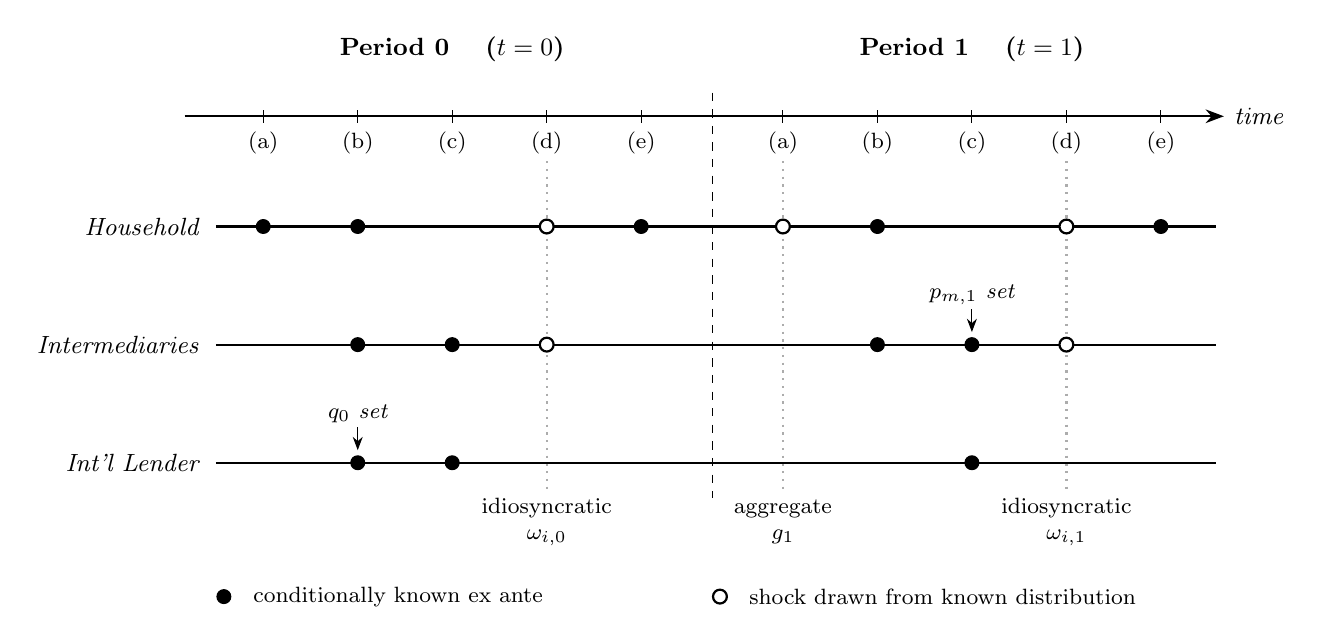
\begin{tikzpicture}[
    >=Stealth,
    every node/.style={font=\small},
    known/.style={circle, draw=black, fill=black, inner sep=0pt, minimum size=5pt},
    shock/.style={circle, draw=black, fill=white, inner sep=0pt, minimum size=5pt, thick},
    agentlbl/.style={anchor=east, font=\small\itshape},
    evlbl/.style={font=\footnotesize},
    periodlbl/.style={font=\bfseries\small},
    shocklbl/.style={font=\footnotesize, align=center},
    pricelbl/.style={font=\footnotesize\itshape, anchor=south}
]
% Event x-positions
\def\xzA{1.0}   \def\xzB{2.2}  \def\xzC{3.4}  \def\xzD{4.6}  \def\xzE{5.8}
\def\xsep{6.7}
\def\xoA{7.6}   \def\xoBC{8.8} \def\xoD{10.0} \def\xoE{11.2} \def\xoF{12.4}
\def\xmax{13.2}
% y-positions
\def\yH{0}     \def\yB{-1.5}  \def\yL{-3.0}
\def\ytop{1.4}
\def\yshock{-3.75}
\def\ykey{-4.7}
% Main timeline arrow
\draw[->, thick] (0, \ytop) -- (\xmax, \ytop)
    node[right, font=\small\itshape] {time};
% Period separator (extends down past shock labels)
\draw[dashed, black] (\xsep, \ytop+0.3) -- (\xsep, \yshock+0.3);
% Period labels
\node[periodlbl] at ({(\xzA+\xzE)/2}, \ytop+0.85) {Period 0 \;\; ($t=0$)};
\node[periodlbl] at ({(\xoA+\xoF)/2}, \ytop+0.85) {Period 1 \;\; ($t=1$)};
% Event tick marks and (a)-(e) labels on main timeline
\foreach \x/\lab in {\xzA/{(a)}, \xzB/{(b)}, \xzC/{(c)}, \xzD/{(d)}, \xzE/{(e)},
                     \xoA/{(a)}, \xoBC/{(b)}, \xoD/{(c)}, \xoE/{(d)}, \xoF/{(e)}} {
  \draw (\x, \ytop-0.08) -- (\x, \ytop+0.08);
  \node[evlbl, below] at (\x, \ytop-0.08) {\lab};
}
% Shock dotted lines - running from just under time arrow all the way through agents down to shock labels
\draw[dotted, thick, gray!65] (\xzD, \ytop-0.57) -- (\xzD, \yshock+0.4);
\draw[dotted, thick, gray!65] (\xoA, \ytop-0.57) -- (\xoA, \yshock+0.4);
\draw[dotted, thick, gray!65] (\xoE, \ytop-0.57) -- (\xoE, \yshock+0.4);
% Agent axes
\draw[thick] (0.4, \yH) -- (\xmax-0.1, \yH);
\draw[thick] (0.4, \yB) -- (\xmax-0.1, \yB);
\draw[thick] (0.4, \yL) -- (\xmax-0.1, \yL);
% Agent labels
\node[agentlbl] at (0.3, \yH) {Household};
\node[agentlbl] at (0.3, \yB) {Intermediaries};
\node[agentlbl] at (0.3, \yL) {Int'l Lender};
% --- Households
\node[known] at (\xzA, \yH) {};
\node[known] at (\xzB, \yH) {};
\node[shock] at (\xzD, \yH) {};
\node[known] at (\xzE, \yH) {};
\node[shock] at (\xoA, \yH) {};
\node[known] at (\xoBC, \yH) {};
\node[shock] at (\xoE, \yH) {};
\node[known] at (\xoF, \yH) {};
% --- Intermediaries
\node[known] at (\xzB, \yB) {};
\node[known] at (\xzC, \yB) {};
\node[shock] at (\xzD, \yB) {};
\node[known] at (\xoBC, \yB) {};
\node[known] at (\xoD,  \yB) {};
\node[shock] at (\xoE,  \yB) {};
% --- International Lender
\node[known] at (\xzB, \yL) {};
\node[known] at (\xzC, \yL) {};
\node[known] at (\xoD, \yL) {};
% --- Price-determination annotations with connector ticks pointing to the relevant node
\node[pricelbl] at (\xzB, \yL+0.38) {$q_0$ set};
\draw[->, thin] (\xzB, \yL+0.45) -- (\xzB, \yL+0.16);
\node[pricelbl] at (\xoD, \yB+0.38) {$p_{m,1}$ set};
\draw[->, thin] (\xoD, \yB+0.45) -- (\xoD, \yB+0.16);
% --- Shock labels attached to the dotted guide lines
\node[shocklbl] at (\xzD, \yshock) {idiosyncratic\\$\omega_{i,0}$};
\node[shocklbl] at (\xoA, \yshock) {aggregate\\$g_1$};
\node[shocklbl] at (\xoE, \yshock) {idiosyncratic\\$\omega_{i,1}$};
% --- Key (below the shock labels)
\node[known] at (0.5, \ykey) {};
\node[anchor=west, font=\footnotesize] at (0.75, \ykey)
    {conditionally known ex~ante};
\node[shock] at (6.8, \ykey) {};
\node[anchor=west, font=\footnotesize] at (7.05, \ykey)
    {shock drawn from known distribution};
\end{tikzpicture}%
}
\caption{Within-period sequence of events by agent, with nodes denoting actions undertaken by a respective agent type within the given sub-period. Labels (a)--(e) correspond to
those above in Section~\ref{sec:timings}.}
\label{fig:timeline}
\end{figure}

\subsection{The Economy} \label{sec:economy}

The model is posed in real terms\footnote{A formal statement of the underlying nominal-neutrality result is given in Appendix~\ref{ap:nominal}.}. The household receives a per-period endowment of $y_t$, expressed in units of domestic inputs. The Period 0 endowment is fixed, whereas the Period 1 endowment process is stochastic, the growth of which $g_1 \equiv y_1/y_0$ follows an AR(1) process in logs\footnote{In simulation of the two-period model, $g_0$ is pinned down parametrically according to historical growth rates, see Section~\ref{sec:quantitative}.}:
\begin{equation}\label{eq:endowgrowth}
\log(g_1) = (1-\rho)\log(\mu_g) + \rho \log(g_0) + \varepsilon, \qquad \varepsilon \sim \mathcal{N}(0, \sigma_g^2).
\end{equation}

There exists an exogenous risk-free gross world interest rate $R^*>1$\footnote{The domestic interest rate collapses to this world rate $R^*$ due to the model's nominal neutrality; see Appendix \ref{ap:nominal}.}. Following \citet{eaton_debt_1981}, the international lender has access to a frictionless world capital market at this rate. As such, the lender will only participate in lending activities, both interperiod and intraperiod, which guarantee them a rate of return at least as high as this market rate.

\subsection{The Domestic Household} \label{sec:household}

The representative household has time-separable expected utility over consumption,
\begin{equation}\label{eq:V0}
V_0 = u(C_0) + \beta \, \E_0\bigl[u(C_1)\bigr],
\end{equation}
where $u$ is strictly increasing, strictly concave, and satisfies Inada conditions, and $\beta \in (0,1)$ is the subjective discount factor. It acts as both a consumer and a final-goods producer, aggregating domestic $\md_t$ and foreign $\mf_t$ inputs via a CES technology,
\begin{equation}\label{eq:CES}
C_t = \bigl[\alpha (\md_t)^{\eta} + (1-\alpha)(\mf_t)^{\eta}\bigr]^{1/\eta}, \qquad t \in \{0,1\},
\end{equation}
where $\alpha \in (0,1)$ is the Armington weight on domestic inputs and $\eta < 0$ governs the elasticity of substitution $\sigma = 1/(1-\eta) \in (0,1)$.

In Period 0, the household acts as the sovereign, issuing non-contingent claims on future consumption $b_1$ that mature in the next period (external debt). In the subsequent Period 1, after the realisation of the endowment shock, the household then selects the haircut $D$ applied to outstanding claims.

\paragraph{Period 0} The household chooses domestic inputs $\md_0$, foreign inputs $\mf_0$, and bond issuance $b_1$ to maximise its lifetime value function \eqref{eq:V0}, subject to its Period 0 budget constraint:
\begin{equation}\label{eq:bc0}
\md_0 + p_{m,0}\,\mf_0 = y_0 - b_0 + q_0 b_1 + \Pi_0,
\end{equation}
where $b_0$ denotes ex-ante fixed pre-existing debt obligations and $\Pi_t$ is a lump-sum dividend received from the domestic intermediary sector, defined in Section~\ref{sec:optimality}. In its debt issuance decision, the household anticipates its optimal Period 1 default policy, thus selecting a $b_1$ that is consistent with its anticipated haircut. Notably, the household acts as a price-taker in its own debt issuance, and does not internalise how its default policy nor issuance impacts its borrowing costs. I seek here to represent coordination failure among dispersed borrowers\footnote{In a unitary-sovereign formulation, the household would internalise the full bond-price schedule, taking into account that issuing more debt depresses the price on all outstanding claims. Sovereign debt in reality is issued on behalf of dispersed beneficiaries (households, firms, a segmented government) whose individual stake in the equilibrium price is small. The aggregate effect of issuance on the bond price is therefore an external cost that no individual perceives \citep{bianchi_overborrowing_2011}, generating over-borrowing relative to the constrained-efficient benchmark \citep{aguiar_economics_2021}. Section~\ref{sec:planner} formalises this externality in Corollary~\ref{prop:overborrowing}. Higher issuance raises the probability and severity of default, which depresses the bond price and erodes the revenue raised on existing claims. This promotes a debt-overhang property \citep{myers_determinants_1977}; the treatment in this thesis being a similar application to sovereign borrowing to that of \citet{goodhart_debt_2018}.}. 

\paragraph{Period 1} After $y_1$ is realised, the household selects the haircut $D \in [0, b_1]$ and input pair $(\md_1, \mf_1)$ to maximise its Period 1 utility in consumption,
\begin{equation}\label{eq:hh_p1}
\max_{D \in [0,b_1],\; \md_1 \geq 0,\; \mf_1 \geq 0} \; u(C_1),
\end{equation}
subject to its Period 1 budget constraint,
\begin{equation}\label{eq:bc1}
\md_1 + p_{m,1}(D) \cdot \mf_1 = y_1 - (b_1 - D) + \Pi_1.
\end{equation} % SPELL IT OUT: why doesn't the household default? define how p_m works (in D), define later 
The household's choice of haircut $D$ has a direct budgetary benefit by providing additional resources for consumption, but also induces an indirect cost, transmitted through the price of imports $p_{m,1}$. The mechanism for this cost, along with the function form of $p_{m,t}$ are formally introduced in Section~\ref{sec:intermediary}. The pathway acts via the domestic intermediaries' holdings of household debt: intermediaries purchase $\gamma$ proportion of $b_1$, thus the larger the haircut the more intermediary balance sheets are eroded, disrupting intermediation of imports and increasing their real cost. The household internalises this price as the primary cost of default in its selection of $D$\footnote{This asymmetric internalisation, when compared to the household's treatment of bond price, is borne out of the long-term debt formulation of my framework: $p_{m,t}$ is contemporaneous in nature, entering directly into the household's budget constraint. $q_0$, on the other hand, is a ``sunk-cost", deriving its price in expectation. A discussion of this asymmetry is available in \citet{aguiar_take_2019}, and my treatment mirrors that of \citet{mendoza_general_2012, goodhart_debt_2018}.}, preventing the household from optimally defaulting on all of its Period 0 debt.

\subsubsection*{Household Optimality}

\paragraph{Intratemporal Optimality} The first-order conditions with respect to $\md_t$ and $\mf_t$ from the CES aggregator \eqref{eq:CES} yield the standard intratemporal demand function:
\begin{equation}\label{eq:mf_demand}
\mf_t = \md_t \left(\frac{1-\alpha}{\alpha\, p_{m,t}}\right)^{\!\frac{1}{1-\eta}},
\end{equation}
in which the foreign-input share rises with the relative price of domestic inputs. As $\eta < 0$ (gross complementarity), the elasticity of substitution $\sigma = 1/(1-\eta) \in (0,1)$ is bounded below unity. The household therefore cannot freely substitute away from foreign inputs when their price rises, and import compression is costly in real consumption terms. 

The shadow value of an additional unit of period $t$ income is
\begin{equation}\label{eq:shadow}
\lambda_t = u'(C_t)\,\frac{\partial C_t}{\partial \md_t} = u'(C_t)\,\alpha\!\left(\frac{C_t}{\md_t}\right)^{\!1-\eta}.
\end{equation}

\paragraph{Optimal Default}

Differentiating the Period 1 Lagrangian with respect to $D$ yields the household's optimal-default first-order condition:
\begin{equation}\label{eq:foc_D}
\frac{\partial \mathcal{L}_1}{\partial D} = \lambda_1\!\left(1 - \mf_1\, \frac{\partial p_{m,1}}{\partial D}\right).
\end{equation}
The marginal benefit is one unit of budget relief, and the marginal cost is the induced increase in the import price $\partial p_{m,1}/\partial D$, weighted by the quantity of imports $\mf_1$ the household purchases. The optimum haircut is governed by the Kuhn–Tucker (KT) conditions over $D \in [0, b_1]$:
\begin{equation}\label{eq:KT}
\begin{cases}
D = 0 & \text{if } 1 \leq \mf_1 \dfrac{\partial p_{m,1}}{\partial D}\bigg|_{D=0} \quad \text{(no default)},\\[10pt]
1 = \mf_1 \dfrac{\partial p_{m,1}}{\partial D} & \text{if } D \in (0, b_1) \quad \text{(partial default)},\\[10pt]
D = b_1 & \text{if } 1 \geq \mf_1 \dfrac{\partial p_{m,1}}{\partial D}\bigg|_{D=b_1} \quad \text{(full default)}.
\end{cases}
\end{equation}
When the marginal cost of even the first unit of default exceeds its budgetary benefit, the household repays in full. When the marginal cost of default is below its benefit, the household repudiates entirely. In the interior region, the household chooses an interior haircut $D \in (0, b_1)$ that balances the two margins. The shape of the marginal-cost schedule $\mf_1 \cdot \partial p_{m,1}/\partial D$ is the central object determining the convexity of import compression in haircut size, which is documented formally in Section~\ref{sec:optimality}.

\paragraph{Intertemporal Optimality}
The household's first-order condition with respect to $b_1$, applying the envelope theorem to $V_1$, yields:
\begin{equation}\label{eq:euler}
\lambda_0\, q_0 = \beta\,\E_0\!\left[\lambda_1\!\left(1 + \gamma\,\mf_1 \frac{\partial p_{m,1}}{\partial N_1}\right)\right].
\end{equation}

The left-hand side of captures the marginal utility cost of issuing one unit of debt at price $q_0$ in Period 0. The right-hand side comprises of the direct utility lost via repayment of one unit of resources, and the indirect effect on Period 1 import prices from the additional net worth that $\gamma$ units of bond holdings deliver to intermediaries. This net-worth dynamic is developed fully in Section~\ref{sec:optimality}, where it is demonstrated that $\partial p_{m,1}/\partial N_1 < 0$, and as such the term $\gamma \mf_1 (\partial p_{m,1}/\partial N_1)$ is strictly negative. Thus, higher debt issuance strengthens bank balance sheets but also increases the household's future repayment burden.

\subsection{Domestic Intermediaries}\label{sec:intermediary}

A continuum of ex-ante identical domestic intermediaries $i \in [0,1]$ operate in a perfectly competitive market with free entry and exit to intermediate foreign inputs $\mf$ in each period. Each intermediary purchases imports using a combination of its own net worth $n_{i,t}$ and working capital $\kappa_{i,t}$ borrowed from the international lender at gross intra-period rate $Z_{i,t}$, with repayment due within the same period. The intermediary's intra-period balance sheet is
\begin{equation}\label{eq:balsheet}
 \mf_{i,t} = n_{i,t} + \kappa_{i,t}, \qquad t \in \{0,1\}.
\end{equation}
It is worth emphasising that $\kappa_{i,t}$ is an intra-period contract, with borrowing and repayment occurring within the same period $t$, distinct from the inter-period sovereign bond $b_1$ issued in Period 0 and maturing in Period 1. The international lender's opportunity cost is $\Rstar$ for both contracts, but the two markets clear independently.

The intermediaries hold $\gamma$ proportion of the household's debt, and as such their net-worth depends on the period and the sovereign's selected haircut:
\begin{align}
n_{i,0} &= \bar{n}(\gamma) + \gamma b_0 - \gamma q_0 b_1, \label{eq:nw0}\\
n_{i,1} &= \bar{n}(\gamma) + \gamma(b_1 - D). \label{eq:nw1}
\end{align}
The sovereign-independent component $\bar{n}(\gamma) > 0$ represents the intermediary sector's exogenous capitalisation. To distinguish the portfolio composition role of $\gamma$ from a mechanical balance-sheet size effect, ex-ante total intermediary assets at the start of Period 0 are $\gamma$-invariant:
\begin{equation}\label{eq:nbar_rescale}
\bar{n}(\gamma) + \gamma b_0 \;\equiv\; \bar{A},
\end{equation}
where $\bar{A}$ is a calibrated constant pinned down by the baseline values $(\bar{n}_{\text{base}}, \gamma)$ in Table~\ref{tab:calibration}. Holding $\bar{A}$ fixed when varying $\gamma$ ensures that comparative statics in $\gamma$ isolate how exposed banks are to sovereign risk, rather than how large their balance sheet is.

Before delivering inputs to the household, each intermediary is subject to an idiosyncratic productivity shock that impacts the amount of effective units of imports they can deliver to the household. Some intermediaries who receive favourable draws will deliver more than expected; some will deliver less under unfavourable draws. Modelled following the ``risk-shock" structure proposed by \citet{christiano_risk_2014} the multiplicative shock $\omega_{i,t}$ is drawn independently each period from a log-normal distribution with mean 1 and variance $\sigma_\omega^2$:
\begin{equation}\label{eq:omega_dist}
\log(\omega_{i,t}) \sim \mathcal{N}\!\left(-\tfrac{\sigma_\omega^2}{2},\, \sigma_\omega^2\right).
\end{equation}

with $F(\omega)$ and $f(\omega)$ denoting the CDF and PDF of this distribution, respectively. As such, the effective foreign inputs delivered to the household are
\begin{equation}\label{eq:agg_supply}
\Mf_t = \int_0^1 \omega_{i,t}\,\mf_{i,t}\,di.
\end{equation}
The parameter $\sigma_\omega$ here is the structural source of financial fragility in the model. It governs the dispersion of intermediary outcomes, and through that dispersion, the curvature of the friction the lender faces. 

The realisation of this shock determines which intermediaries are able to sufficiently honour their working-capital obligation to the international lender; an intermediary with a sufficiently low shock draw will not deliver enough effective import units to cover repayment $Z_{i,t}\kappa_{i,t}$, thus they are forced into bankruptcy. Let $\bar{\omega}\geq 0$ denote the shock \textit{cutoff threshold}, which corresponds to the exact shock realisation at which the intermediary just breaks even:
\begin{equation}\label{eq:threshold}
\bar{\omega}\, p_{m,t}\, \mf_{i,t} = Z_{i,t}\,\kappa_{i,t} = Z_{i,t}\bigl( \mf_{i,t} - n_{i,t}\bigr).
\end{equation}
If $\omega_{i,t} \geq \bar{\omega}$, the intermediary repays in full and retains the surplus. If $\omega_{i,t} < \bar{\omega}$, the intermediary fails; the lender pays an auditing cost which destroys a fraction $\mu$ of realised assets in order to verify the state of the intermediary\footnote{The lender therefore recovers $(1-\mu)\omega_{i,t}\,p_{m,t}\,\mf_{i,t}$.}. This threshold $\bar \omega$ acts as a primary structural object, linking the level of financial fragility within the economy to the intermediary balance sheets, expected lender payoff and ultimately import costs faced by the household. 

\paragraph{Intermediary Optimality} Each intermediary chooses $\mf_{i,t}$ to maximise expected profits, net of the lender's claim,
\begin{equation}\label{eq:int_obj}
\max_{\mf_{i,t}} \; \bigl[1 - \Gamma(\bar{\omega})\bigr]\,p_{m,t}\,\mf_{i,t},
\end{equation}
where $\Gamma({\bar \omega})$ denotes the expected gross revenue share to the lender, defined formally in Section~\ref{sec:lender}. The intermediary problem yields the first-order condition
\begin{equation}\label{eq:int_foc}
\bigl[1 - \Gamma(\bar{\omega})\bigr]\,p_{m,t}\,\mf_{i,t} = \Gamma'(\bar{\omega})\,Z_{i,t}\,n_{i,t}.
\end{equation}
Unlike the bilateral optimal contract in \citet{christiano_risk_2014}, intermediaries here take $Z_{i,t}$ as given in a competitive credit market. They do not internalise the marginal auditing costs when choosing their scale of intermediation, generating a steeper external finance premium for a given level of net worth.

% requires further discussion

\paragraph{Intermediary dividends.} All intermediaries are owned by the representative household, who acts as the residual claimant on any surplus they generate. Once the idiosyncratic shock is realised and obligations to the international lender are settled, solvent intermediaries distribute their surplus revenue as a lump-sum dividend\footnote{The per-unit surplus of intermediary $i$, net of working-capital repayment, is $\pi_{i,t} = (\omega_{i,t} - \bar{\omega}_t)\,p_{m,t}\,\mf_{i,t} \quad \text{if } \omega_{i,t} \geq \bar{\omega}_t, \quad 0 \text{ otherwise}.$}. Aggregating across the continuum of intermediaries and applying the law of large numbers:
\begin{equation}\label{eq:Pi_agg}
\Pi_t = \int_{\bar{\omega}_t}^{\infty} (\omega - \bar{\omega}_t)\,p_{m,t}\,\Mf_t\,dF(\omega) = \bigl[1 - \Gamma(\bar{\omega}_t)\bigr]\,p_{m,t}\,\Mf_t.
\end{equation}
This is the aggregate dividend $\Pi_t$ that enters the household's budget constraints \eqref{eq:bc0} and \eqref{eq:bc1}.

% Discussion needed: provide a genuine microfoundation (heterogeneous bank ownership, atomistic-shareholder informational frictions, distinct ownership or policy agents)

\subsection{International Lender} \label{sec:lender}

The international lender is risk-neutral, infinitely funded, and prices all contracts at the risk-free rate $\Rstar$. It participates in two markets within the economy: the intra-period working-capital market, in which it lends to domestic intermediaries, and the inter-period sovereign bond market, in which it holds a fraction $1-\gamma$ of the household's debt. These markets both share an opportunity cost of capital of $R^*$, but are structurally distinct.

\paragraph{Working capital market.} The lender extends working capital loans $\kappa_{i,t}$ to each intermediary at the start of the period, with repayment from the intermediary's realised import revenue at the period's close. The lender, however, is subject to a CSV friction \citep{townsend_optimal_1979, bernanke_chapter_1999}; it cannot costlessly observe the intermediary's realised productivity shock $\omega_{i,t}$ ex-post. To verify the outcome of any individual intermediary, an auditing cost must be paid equal to fraction $\mu \in (0,1)$ of the intermediary's realised assets.
Under the optimal debt contract, the lender collects the contractual payment $\bar{\omega}\,p_{m,t}\,\mf_{i,t}$ from intermediaries drawing $\omega_{i,t} \geq \bar{\omega}$, and audits intermediaries drawing $\omega_{i,t} < \bar{\omega}$, recovering the residual $(1-\mu)\,\omega_{i,t}\,p_{m,t}\,\mf_{i,t}$. The lender's expected gross revenue share, expressed per unit of intermediated imports, is
\begin{equation}\label{eq:Gammadef}
\Gamma(\bar{\omega}) \equiv \int_0^{\bar{\omega}} \omega \, dF(\omega) + \bar{\omega}\bigl[1 - F(\bar{\omega})\bigr],
\end{equation}
The first term captures partial recovery from defaulting intermediaries, with the second term representing the full repayment mass from solvent intermediaries at the upper tail of the risk-shock distribution. The portion of revenue arising from failed intermediaries is
\begin{equation}\label{eq:Gdef}
G(\bar{\omega}) \equiv \int_0^{\bar{\omega}} \omega \, dF(\omega),
\end{equation}
so that $\mu G(\bar{\omega})$ is the expected deadweight loss the lender must absorb that arises from state-verification. As such, the net surplus accruing to the lender per unit of intermediated imports is $\Gamma(\bar{\omega}) - \mu G(\bar{\omega})$, the lender's gross revenue share net of verification cost. This object is the central reduced-form characterisation of the financial friction, recurring throughout the thesis.

These contracting objects satisfy intuitive properties, namely, (i) $\Gamma'(\bar{\omega}) = 1 - F(\bar{\omega}) > 0$: a marginal increase in the threshold raises the lender's expected revenue by the share of intermediaries that remain solvent, and; (ii) $G'(\bar{\omega}) = \bar{\omega} f(\bar{\omega}) \geq 0$: a marginal increase in the threshold raises expected revenue from defaulting intermediaries by the value of the failed intermediary at the margin, weighted by the density of intermediaries over the threshold. The most important property for deriving convexity in default costs, however, is (iii) $\Gamma''(\bar \omega)=-f(\bar \omega)$: the lender's expected revenue is concave in the threshold, as the share of solvent intermediaries decreases. Combining these properties, one can see that the lender's net surplus $\Gamma(\bar{\omega}) - \mu G(\bar{\omega})$ is non-monotone in the cutoff threshold; as $\bar \omega$ rises, both $\Gamma$ and $\mu G$ rise, but at sufficiently high threshold values $\mu G$ does so at a faster rate. The latter dead-weight term eventually dominates, crucially generating \textit{structural non-linearity} within the external finance premium. This convexity propagates throughout the doom-loop. 

Competition between international lenders drives the working-capital contract down to a zero-profit condition: the expected net surplus must equal the opportunity cost of capital. Thus, the lender's participation constraint is
\begin{equation}\label{eq:lender_zp}
\bigl[\Gamma(\bar{\omega}) - \mu G(\bar{\omega})\bigr]\,p_{m,t}\,\mf_{i,t} = \Rstar\bigl( \mf_{i,t} - n_{i,t}\bigr).
\end{equation}
The left-hand side is the lender's expected payoff per period, the right-hand side is the opportunity cost of the working capital loaned to the intermediaries, $\kappa_{i,t} = \mf_{i,t} - n_{i,t}$. The constraint pins down the equilibrium relationship between the threshold $\bar{\omega}$, the price of imports $p_{m,t}$, and the level of intermediary leverage in the economy.

\paragraph{Intertemporal bond market.} The lender holds $1-\gamma$ share of the household's outstanding debt $b_1$. The lender's payoff in purchasing these bonds is state-contingent; the household selects the haircut $D$ after realisation of the aggregate endowment shock, and the lender receives $b_1-D(y_1,b_1)$ per unit of debt held\footnote{In this formulation, the lender is unable to recover any of the portion of debt defaulted upon. Introducing a recovery rate would simply rescale the equilibrium level of debt issuance, leaving the mapping between the haircut and real allocations and prices unchanged. Here, I am following similar treatment by \citep{eaton_debt_1981, arellano_default_2008}.}. The risk neutrality of the lender and the competitive international lending market imply that the lender prices household debt at the zero-profit expected recovery rate,
\begin{equation}\label{eq:bondprice}
q_0(y_0, b_1) = \frac{1}{\Rstar}\,\E_0\!\left[1 - \frac{D(y_1, b_1)}{b_1}\right].
\end{equation}

Here, the lender acts with rationality in its pricing decision, and observes that the atomistic household does not internalise $q_0$ in its debt issuance.

%========================================================================
\section{Equilibrium Definitions} \label{sec:equilibrium}
%========================================================================

\subsection{Aggregation and Market Clearing}

Because all intermediaries are ex-ante identical, in any symmetric equilibrium they hold the same net worth ($n_{i,t} = N_t$), purchase the same raw imports ($\mf_{i,t} = \Mf_t$), borrow the same working capital ($\kappa_{i,t} = K_t$), and face the same default threshold ($\bar{\omega} = \bar{\omega}_t$). Henceforth all intermediary-level variables are written without the $i$ subscript.

Three markets must clear in equilibrium. Firstly, the sovereign debt market requires that total issuance equals total demand\footnote{Formally, $b_1 = \gamma b_1 + (1-\gamma)b_1$.}, with intermediaries holding $\gamma b_1$ and the international lender holding $(1-\gamma)b_1$. Second, the foreign inputs market requires that the household's demand for effective foreign inputs equals aggregate intermediary supply net of auditing losses:
\begin{equation}\label{eq:mc_foreign}
\mf_t = \Mf_t\bigl[1 - \mu G(\bar{\omega}_t)\bigr].
\end{equation}
Third, the domestic inputs market clears by Walras' law given the first two conditions and the household budget constraint. The balance-of-payment constraints are written in Appendix \ref{ap:balance-of-payments}.

\subsection{Equilibrium Definition}

\begin{definition}[Competitive Equilibrium]\label{def:equil}
Given initial debt $b_0$, long-run net worth $\bar{n}$, exogenous global parameter $R^*$ and realised aggregate endowments $(y_0, y_1)$, a competitive equilibrium is defined as a collection of prices $\{q_0,\, p_{m,0},\, p_{m,1},\, Z_0,\, Z_1\}$, thresholds $\{\bar{\omega}_0,\, \bar{\omega}_1\}$, and allocations $\{C_t,\, \md_t,\, \mf_t,\, \Mf_t,\, b_1,\, D,\, N_t,\, K_t,\, \Pi_t\}_{t=0,1}$ such that:
\begin{enumerate}[label=(\roman*)]
\item The representative household optimises lifetime utility, choosing $(\md_t, \mf_t, b_1, D)$ given prices $(q_0, p_{m,0}, p_{m,1})$;
\item Each domestic intermediary selects $\mf_{i,t}$ to maximise expected profit \eqref{eq:int_obj}, given the lending rate $Z_t$;
\item The international lender prices sovereign bonds via \eqref{eq:bondprice} and the working capital zero-profit condition \eqref{eq:lender_zp} holds; % be explicity - what?
\item The sovereign debt, foreign input, and domestic input markets clear;
\item Net worth satisfies \eqref{eq:nw0}--\eqref{eq:nw1}, working capital is consistent: $K_t =  \Mf_t - N_t$, and aggregate dividends satisfy \eqref{eq:Pi_agg}. % nothing else other than markets - no optimisation
\end{enumerate}
\end{definition}

%========================================================================
\section{The Financial Friction} \label{sec:optimality}
%========================================================================

Here, I combine the intermediaries' optimisation problem with the lender's participation constraint to derive the central financial friction objects of the model, via which the default costs propagate through the real economy and form the central ``doom loop" mechanism. These objects are (i) the external finance premium, capturing the wedge between the lending rate and the world rate; (ii) the equilibrium leverage-threshold relationship, which pins down the failure threshold $\bar\omega$ as a function of intermediary leverage; and (iii) the import-price equation, which relates intermediary leverage and the cutoff threshold to the import price the household faces. The convexity result, established as Proposition~\ref{prop:convexity} below, is the main theoretical contribution of this thesis; it microfounds the empirically documented relationship between haircut severity and disproportionate consumption losses (Section~\ref{sec:intro}) which stems from the CSV friction originating from financial intermediation.

Firstly, I derive the \textit{external finance premium}, capturing how the CSV friction increases the gross-interest rate the intermediaries face, in excess of the world rate. Aggregating across intermediaries and dividing the threshold condition \eqref{eq:threshold} by the zero-profit condition \eqref{eq:lender_zp}, the equilibrium lending rate satisfies
\begin{equation}\label{eq:efp}
Z_t = \Rstar \cdot \underbrace{\frac{\bar{\omega}_t}{\Gamma(\bar{\omega}_t) - \mu G(\bar{\omega}_t)}}_{\text{external finance premium}}.
\end{equation}
The ratio $Z_t / \Rstar$ exceeds unity whenever $\bar{\omega}_t > 0$, and is increasing in $\bar{\omega}_t$\footnote{In order to prevent friction in the household's Period 0 consumption, and form a baseline for Period 1 allocations, I impose the assumption herein that intermediaries are sufficiently well capitalised in Period 0, such that the external finance premium is negligible; $p_{m,0} \approx  \Rstar$.}. Dividing the intermediary FOC \eqref{eq:int_foc} by the zero-profit condition \eqref{eq:lender_zp} and substituting the external finance premium \eqref{eq:efp}, I derive the \textit{leverage-threshold condition},
\begin{equation}\label{eq:omega_leverage}
1 - \Gamma(\bar{\omega}_t) = \Gamma'(\bar{\omega}_t)\,\bar{\omega}_t \cdot \frac{N_t}{ \Mf_t - N_t}.
\end{equation}
This condition demonstrates that the cutoff threshold $\bar{\omega}_t$ is pinned down by the leverage ratio of the intermediaries in equilibrium alone. The propogation of the threshold throughout the default cost transmission chain, therefore, wholly stems from the level of bank capitalisation.

Solving the zero-profit condition \eqref{eq:lender_zp} for $p_{m,t}$ yields the \textit{import-price equation},
\begin{equation}\label{eq:pm}
p_{m,t} =  \Rstar \cdot \underbrace{\left(1 - \frac{N_t}{ M^f_t}\right)}_{\text{leverage}} \cdot \underbrace{\frac{1}{\Gamma(\bar{\omega}_t) - \mu G(\bar{\omega}_t)}}_{\text{CSV friction}}.
\end{equation}

The price of imports are subject to a wedge stemming from the external finance premium. Intermediary leverage scales the wedge, whereas the CSV friction, the inverse of the lender's net surplus per unit of intermediated imports, provides the wedge convexity in the cutoff threshold. As established in Section~\ref{sec:lender}, this surplus is non-monotone in the threshold. In order to restrict attention to the local region of the CSV friction suitable for a financially distressed economy, I impose the following, herein,

\begin{assumption} \label{ass:operating_region}
    Assume the CSV friction operates within the high-leverage region where the lender's net surplus is locally \textit{decreasing} in the cutoff threshold, that is, $[\Gamma' - \mu G'] < 0$.\footnote{This region characterises the financially-distressed regime relevant to default analysis; it is the region in which \citet{bernanke_chapter_1999} ``financial accelerator" amplification operates, and is the region informally induced by Assumption~\ref{ass:interior}.}
\end{assumption}

The reciprocal of \eqref{eq:pm} therefore accelerates as the net surplus contracts, generating nonlinear price response to changes in intermediary balance sheets, as pinned down by the leverage threshold condition \eqref{eq:omega_leverage}.

\begin{remark}
    For the CSV friction to operate within the operating region imposed by Assumption~\ref{ass:operating_region}, $\mu\neq0$. This limiting case $\mu \to 0$ leads to a failure of non-monotonicity in $\Gamma(\bar{\omega}) - \mu G(\bar{\omega})$, flattening the convexity that is a key characteristic in the default cost $p_{m,1}$ necessary to induce import compression. A numerical illustration of this point is written in Section~\ref{sec:mech_decomp}.
\end{remark}


\subsection{Transmission of Default to Import Prices}

The mechanism by which sovereign default raises import prices, our key transmission process of interest, can be traced through the intermediary balance sheets. From the net-worth equation \eqref{eq:nw1}:
\begin{equation}\label{eq:dpm_dD}
\frac{\partial p_{m,1}}{\partial D} = -\gamma \frac{\partial p_{m,1}}{\partial N_1}.
\end{equation}
Combining this with the \textit{leverage-threshold condition} and the \textit{import-price equation}, I arrive at the haircut-imports default cost relationship that is central to this thesis. An increase in $D$ erodes intermediary net worth, raising leverage, pushing up the default threshold, increasing the external finance premium, and passing through to the import price:
\[
D \uparrow \;\xrightarrow{\eqref{eq:nw1}}\; N_1 \downarrow \;\xrightarrow{\eqref{eq:omega_leverage}}\; \bar{\omega}_1 \uparrow \;\xrightarrow{\eqref{eq:efp}}\; \frac{Z_1}{\Rstar} \uparrow \;\xrightarrow{\eqref{eq:pm}}\; p_{m,1} \uparrow \;\xrightarrow{\eqref{eq:mf_demand}}\; \mf_1 \downarrow \;\Longrightarrow\; C_1 \downarrow.
\]

The transmission chain delivers a relationship between the haircut $D$ and the import price $p_{m,1}$ whose shape is strictly convex. First, the sensitivity of the cutoff threshold to net worth, $\partial\bar\omega/\partial N$, is itself an increasing function of the level of leverage. As net worth falls and leverage rises, the marginal intermediary tipped into failure carries proportionally larger weight, and the threshold response steepens. Second, the lender's net surplus $\Gamma - \mu G$ contracts as the threshold rises (Section~\ref{sec:lender}). These two effects compound, resulting in a convex pass-through:

\begin{lemma}[Partial-equilibrium import-price response]\label{lem:pe-resp}
Fix $M^f_1$ and let $\bar{\omega}_1$ adjust according to \eqref{eq:omega_leverage}. Then:
\begin{enumerate}
    \item[\textup{(i)}] $\dfrac{\partial \bar{\omega}_1}{\partial N_1}\Big|_{M^f_1} < 0$;
    \item[\textup{(ii)}] $\dfrac{\partial p_{m,1}}{\partial N_1}\Big|_{M^f_1} < 0$;
    \item[\textup{(iii)}] $\left|\dfrac{\partial p_{m,1}}{\partial N_1}\Big|_{M^f_1}\right|$ 
    is strictly increasing in $\bar{\omega}_1$.
\end{enumerate}

Proof: See Appendix~\ref{ap:penalty-convexity}

\end{lemma}

Lemma~\ref{lem:pe-resp} formalises the mechanism underlying the transmission chain of Section~\ref{sec:optimality}. Whilst Lemma~\ref{lem:pe-resp} admits a local partial equilibrium result, I confirm via numerical simulation that convexity in the default penalty holds in general equilibrium:

\begin{proposition}[Convexity of the Default Penalty]\label{prop:convexity}
Consider the mapping $D \mapsto \widetilde{p}_{m,1}(D)$ traced along the Period~1 import transmission chain~\eqref{eq:nw1}--\eqref{eq:pm}, where $\widetilde{p}_{m,1}$ corresponds to $p_{m,1}$ in equilibrium. Under Assumptions~\ref{ass:interior} and~\ref{ass:operating_region}, then:
\begin{enumerate}
    \item[\textup{(i)}] $\widetilde{p}_{m,1}(D)$ is strictly increasing in $D$;
    \item[\textup{(ii)}] $\widetilde{p}_{m,1}$ is strictly convex in $D$.
\end{enumerate}
A linear increase in sovereign default triggers a more-than-proportional increase in 
the domestic import price. Convexity arises from two reinforcing channels: as $D$ rises, 
$|\partial \bar{\omega}_t / \partial N_t|$ grows, as the numerator of $\partial p_{m,t}/\partial N_t$ 
expands while the denominator contracts; and $[\Gamma(\bar{\omega}_t) - \mu G(\bar{\omega}_t)]^2$ 
in the denominator of $\partial p_{m,t}/\partial N_t$ shrinks as $\bar{\omega}_t$ rises. 
Partial-equilibrium signing of the underlying derivatives is established in Lemma~\ref{lem:pe-resp} 
of Appendix~\ref{ap:penalty-convexity}. With reference to Figure~\ref{fig:numeric_feedback}.\footnote{Numerical verification of convexity along the equilibrium follows \citet{arellano_default_2008} for analogous higher-order structural objects.}, the general equilibrium schedule lies strictly above the partial equilibrium schedule for $D > D^{\ast}$, confirming that the equilibrium feedback through $M^f_1$ reinforces the partial equilibrium signing of Lemma~\ref{lem:pe-resp}.
\end{proposition}

Proposition~\ref{prop:convexity} rationalises the primary stylised empirical regularity of this paper: the disproportionate consumption losses, stemming from import compression, associated with larger haircuts. It does so from an endogenous friction in the contracting relationship between heterogeneous domestic intermediaries and international lenders. The convexity does not arise from imposed parametric assumptions about the shape of the default cost.

\begin{figure}
    \centering
    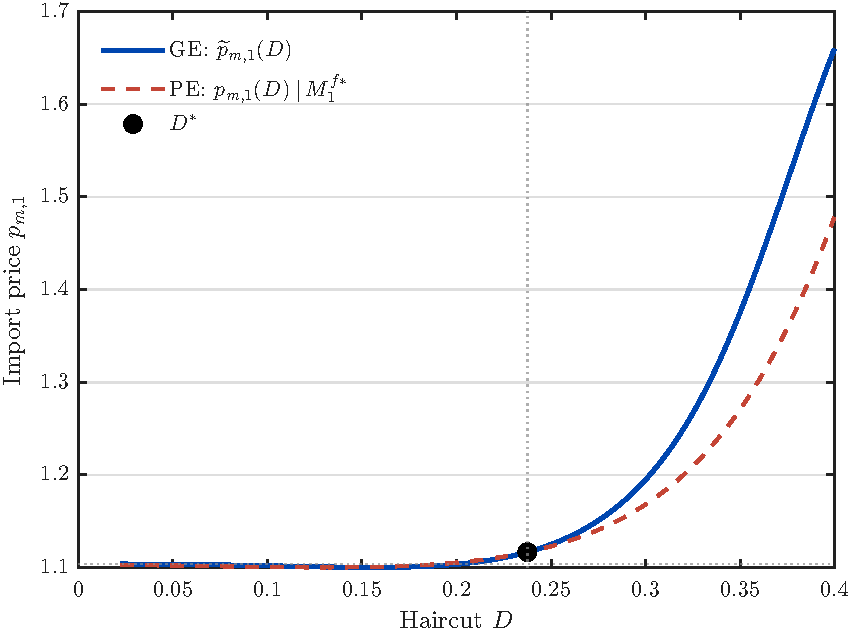
\includegraphics[width=0.75\linewidth]{figure_convexity_small_horizontal.pdf}
    \caption{\textit{Equilibrium import-price schedule $D \mapsto \widetilde{p}_{m,1}(D)$.} The solid line plots the equilibrium import price computed by solving \eqref{eq:sys_leverage}--\eqref{eq:sys_clearing} at each $D$, with $M^f_1$ adjusting endogenously. The dashed line plots the partial-equilibrium response detailed in Lemma~\ref{lem:pe-resp}, holding $M^f_1$ fixed at its equilibrium (under Section~\ref{sec:quantitative} calibration) value $M^{f\ast}_{1}$.}
    \label{fig:numeric_feedback}
\end{figure}

The default penalty also possesses the desirable property of strictly increasing in the inverse of debt-to-GDP, as formalised in Corollary~\ref{corol:inv-debt-gdp} contained within Appendix~\ref{ap:default-cost-debt-proof}. Combining Proposition \ref{prop:convexity} with Corollary \ref{corol:inv-debt-gdp} induces over-borrowing consistent with debt-overhang; a comparative static formalisation of this can be found in Section \ref{sec:implications}.

%========================================================================
\section{Characterisation of Equilibrium} \label{sec:chareq}
%========================================================================

\subsection{Period 1 Equilibrium}

Take as given the states $(y_1, b_1)$ and the parameter $R^*$. 
Define the following shorthand, which depend only on 
$(D, \bar{\omega}_1, M^f_1)$ and parameters:
\begin{align*}
N_1(D) &\equiv \bar{n} + \gamma(b_1 - D), \\
\ell_1(D, M^f_1) &\equiv 1 - \frac{N_1(D)}{M^f_1}, \\
\Psi(\bar{\omega}_1) &\equiv \Gamma(\bar{\omega}_1) - \mu G(\bar{\omega}_1), \\
p_{m,1}(D, \bar{\omega}_1, M^f_1) &= R^* \cdot 
  \frac{\ell_1}{\Psi(\bar{\omega}_1)}.
\end{align*}
The Period~1 equilibrium values of $(D, \bar{\omega}_1, M^f_1)$ 
solve the following nonlinear system:

\medskip
\textit{Leverage--threshold condition} 
[from \eqref{eq:omega_leverage} and \eqref{eq:nw1}]:
\begin{equation}\label{eq:sys_leverage}
1 - \Gamma(\bar{\omega}_1) 
= \Gamma'(\bar{\omega}_1)\,\bar{\omega}_1 
  \cdot \frac{N_1(D)}{M^f_1 - N_1(D)}.
\end{equation}

\textit{Foreign input market clearing} 
[from \eqref{eq:mf_demand}, \eqref{eq:bc1}, 
\eqref{eq:mc_foreign}, and \eqref{eq:Pi_agg}]:
\begin{equation}\label{eq:sys_clearing}
M^f_1 \bigl[1 - \mu G(\bar{\omega}_1)\bigr]
\left[
  \left(\frac{\alpha\, p_{m,1}}{1 - \alpha}\right)^{\!\sigma} 
  + p_{m,1}
\right]
= y_1 - (b_1 - D) 
  + \bigl[1 - \Gamma(\bar{\omega}_1)\bigr]\, p_{m,1}\, M^f_1.
\end{equation}

\textit{Interior default condition} 
[from \eqref{eq:KT}, \eqref{eq:dpm_dD}, 
and \eqref{eq:dpm_dn}]:
\begin{equation}\label{eq:sys_default}
\Psi(\bar{\omega}_1)^2 
= \gamma R^* M^f_1 \bigl[1 - \mu G(\bar{\omega}_1)\bigr]
\left(
  \frac{\Psi(\bar{\omega}_1)}{M^f_1}
  + \ell_1 
    \Psi'(\bar{\omega}_1)
    \left\lvert
      \frac{\partial \bar{\omega}_1}{\partial N_1}
    \right\rvert
\right),
\end{equation}
where
\begin{equation*}
\frac{\partial \bar{\omega}_1}{\partial N_1}
= \frac{
  -\Gamma'(\bar{\omega}_1)\,\bar{\omega}_1\, M^f_1
}{
  (M^f_1 - N_1)
  \Bigl[
    \Gamma'(\bar{\omega}_1)(M^f_1 - N_1)
    + N_1 \bigl[\Gamma''(\bar{\omega}_1)\,\bar{\omega}_1 
      + \Gamma'(\bar{\omega}_1)\bigr]
  \Bigr]
}.
\end{equation*} \\

At corner solutions, \eqref{eq:sys_default} is replaced by $D = 0$ or $D = b_1$ with the corresponding inequality 
from the KT conditions \eqref{eq:KT}. \\

All other Period~1 variables are determined residually: $N_1$ from 
\eqref{eq:nw1}, $p_{m,1}$ from \eqref{eq:pm}, $m^f_1$ from \eqref{eq:mc_foreign}, $\Pi_1$ from \eqref{eq:Pi_agg}, $m^d_1$ from \eqref{eq:bc1}, $C_1$ from \eqref{eq:CES}, $Z_1$ from \eqref{eq:efp}, and $K_1 = M^f_1 - N_1$. \\

\subsection{Period 0 Equilibrium}

Given Period 1 policy functions $D(y_1,b_1)$, and the associated Period 1 equilibrium mappings, the Period 0 equilibrium values of $(b_1, q_0)$ solve the following system: \\

\textit{Euler equation} [from \eqref{eq:euler}]:
\begin{equation}
\lambda_0\, q_0 = \beta\,\E_0\!\left[\lambda_1\!\left(1 + \gamma\,\mf_1 \frac{\partial p_{m,1}}{\partial N_1}\right)\right],
\end{equation}
where $\lambda_t$ is derived in \eqref{eq:shadow}.\\

\textit{Intertemporal bond pricing equation} [from \eqref{eq:bondprice}]:
\begin{equation}
    q_0 = \frac{1}{\Rstar}\,\E_0\!\left[1 - \frac{D(y_1, b_1)}{b_1}\right].
\end{equation}

Given a solution, the remaining Period~0 objects are recovered as: $N_0$ from \eqref{eq:nw0}, $\mf_0$ from 
\eqref{eq:mf_demand}, $\md_0$ from \eqref{eq:bc0}, $C_0$ from \eqref{eq:CES}, $\Pi_0$ from 
\eqref{eq:Pi_agg}, and $K_0 = M^f_0 - N_0$. Under the assumption of sufficient Period 0 intermediary capitalisation, $\bar{\omega}_0$ and $Z_0$ are pinned down by \eqref{eq:omega_leverage} and \eqref{eq:efp} at negligible values of the external finance premium.

\paragraph{Ruling out no-trade equilibrium} For the rest of the thesis, attention will be restricted to the non-trivial interior partial default equilibrium, in which $q_0>0$ and $D\in (0,b_1)$;

\begin{assumption}\label{ass:interior}
Parameters $(\bar{n}, \gamma, \sigma_\omega, \mu, \eta, \alpha, R^*)$ and states $(y_1, b_1)$ are such that the KT conditions~\eqref{eq:KT} admit an interior solution $D \in (0, b_1)$.
\end{assumption}

The model admits a second class of equilibria in which the international lender anticipates full default, sets $q_0=0$, and the household is indifferent between not borrowing and borrowing for free with the intention of defaulting upon all claims, as identified by \citet{dubey_default_2005} in models of default with non-contingent debt. The two-period setting presented in this model, without a continuation value from market access, means that the household is exactly indifferent between these two equilibria. I choose to omit the analysis of such an equilibrium, following the practice of \citet{arellano_default_2008}, \citet{peiris_capital_2025} and others, to focus upon the borrowing, default, and intermediary channels that are of primary interest to this thesis.


%========================================================================
\section{Comparative Statics}\label{sec:implications}
%=======================================================================

Proposition~\ref{prop:convexity} established that the imports-based cost of default is strictly convex in the haircut, with the curvature driven by the contracting friction between domestic banks and international lenders. This section develops two comparative statics that characterise this convexity in financial system structural parameters. First, I show that the share of sovereign debt held by domestic intermediaries, $\gamma$, is the primary parameter governing the strength of the haircut–consumption pass-through, transmitted via $\bar \omega$. The model thus admits a cross-country mapping from financial-sector composition to the haircut-import compression elasticity, an empirical object. Second, I show that the idiosyncratic productivity risk faced by intermediaries, $\sigma$, is both necessary for an interior equilibrium and is itself an amplifier of the convexity. The section concludes by characterising the welfare implications of the debt-issuance externality, where the atomistic household over-borrows relative to a constrained Ramsey planner who internalises the bond-price schedule.

\subsection{Amplification in Domestic Bank Sovereign Debt Exposure}\label{sec:comp_stat_gamma}

As discussed in Section \ref{sec:intermediary}, the comparative static in $\gamma$ isolates the role of domestic bank exposure to sovereign debt. Since $\bar n(\gamma)+\gamma b_0\equiv \bar A$, changes in $\gamma$ should not be interpreted as changes in the size of the banking sector, rather as changes in the composition of intermediary portfolios toward domestic sovereign claims.
 
Sovereign debt exposure scales the sensitivity of the cost of default to the CSV friction throughout the entire transmission chain, to \eqref{eq:pm}, via \eqref{eq:nw1}: $\partial N_1/\partial D = -\gamma$. Higher $\gamma$ amplifies the pass-through from default to intermediary net worth erosion, raising the external finance premium and import price, generating stronger import compression and larger consumption losses conditional on any given haircut. Proposition~\ref{prop:convexity} then implies that the consumption loss conditional on any given haircut is strictly increasing and convex in $\gamma$. Figure~\ref{fig:partial_gamma} illustrates this property numerically, under partial equilibrium. Holding $(y_1, b_1, \sigma_\omega)$ fixed and tracing the contracting friction across forced haircuts, the slope and convexity of EFP and import compression with respect to $D$ both intensify in $\gamma$.

\begin{figure}
    \centering
    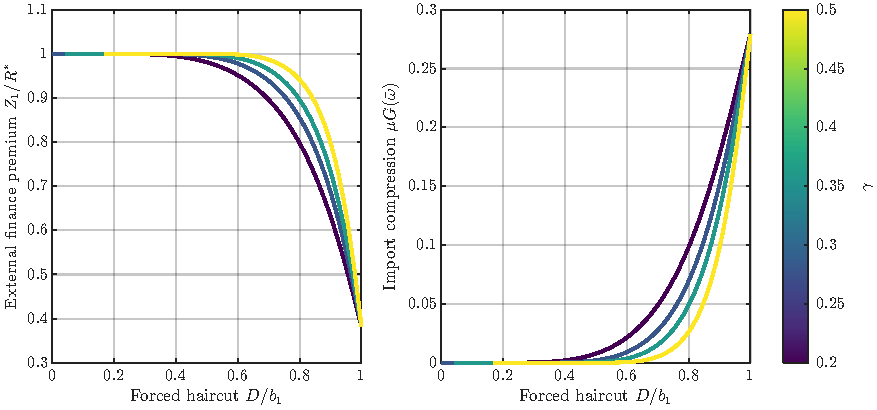
\includegraphics[width=1\linewidth]{partial_equilibrium_small.pdf}
    \caption{Partial equilibrium responses of CSV objects to exogenous shifts in $\gamma$, under $y_1 = 1.0431$ (mean), $b_1 = 0.6244$, $\sigma_{\omega} = 0.25$, and the baseline calibration written in Section~\ref{sec:quantitative}.}
    \label{fig:partial_gamma}
\end{figure}

These comparative statics are intensive-margin results. In an analogous binary-default formulation of this model, $\gamma$ would affect the cost of the household switching from repayment to default, but it would not characterise how the marginal cost curve of default grows in steepness and convexity with the size of the haircut. Here, under partial default, import prices and consumption can be quantitatively mapped to observed haircuts, offering a cross-country mapping. Two countries facing identical aggregate shocks, with identical negotiated haircuts, will experience different real consumption losses in import compression if their banking sectors differ in domestic sovereign exposure. The size of this wedge is itself increasing in the haircut, so the cross-country dispersion in real outcomes is largest in the episodes where haircuts are most severe. This is consistent with the cross-country empirical regularity established by \citet{asonuma_costs_2024}. Countries with deeper bank intermediation transmit sovereign haircuts to household consumption through a sharper, more convex pass-through.

Figure~\ref{fig:cs_haircuts} reports the general-equilibrium expected haircut $\E[D/b_1]$ across $(\gamma, \sigma_\omega)$. The equilibrium haircut is visibly decreasing in $\gamma$ over the relevant support (Ruling out no-trade equilibria, as per Assumption~\ref{ass:interior}). When facing the steeper marginal cost of default that Figure~\ref{fig:partial_gamma} establishes in partial equilibrium, the household chooses to default less. $\gamma$ thus acts as an exogenous commitment device, raising the structural penalty for default and disciplining the chosen haircut in equilibrium. This is an effect that, as Proposition~\ref{prop:internal_default} establishes, $\sigma_\omega$ shares.

At the extensive margin, the model produces a necessity result for domestic banking exposure to sovereign debt to maintain the net-worth channel transmission of default costs. Looking at the limiting case where $\gamma\to0$, intermedary net-worth becomes insensitive to $D$,
\begin{equation*}
    N_1=\bar A, \quad \partial N_1/\partial D=0,
\end{equation*}

causing a collapse in the transmission chain. The KT condition \eqref{eq:KT} reduces to $\partial\mathcal{L}_1/\partial D=\lambda_1>0\quad \forall \space D\in[0,b_1]$ and the corner $D^*=b_1$ is reached in every state. This is an induced no-trade equilibrium of the type ruled out by Assumption~\ref{ass:interior}, and is \textit{state-invariant}. The banking channel is a load-bearing structure for interior default, rather than acting as a scaler akin to \citet{rojas_bright_2024}. A quantitative illustration of equilibrium outcomes in this limiting case, where $\gamma=0$, is written in Section~\ref{sec:mech_decomp}

\begin{figure}
    \centering
    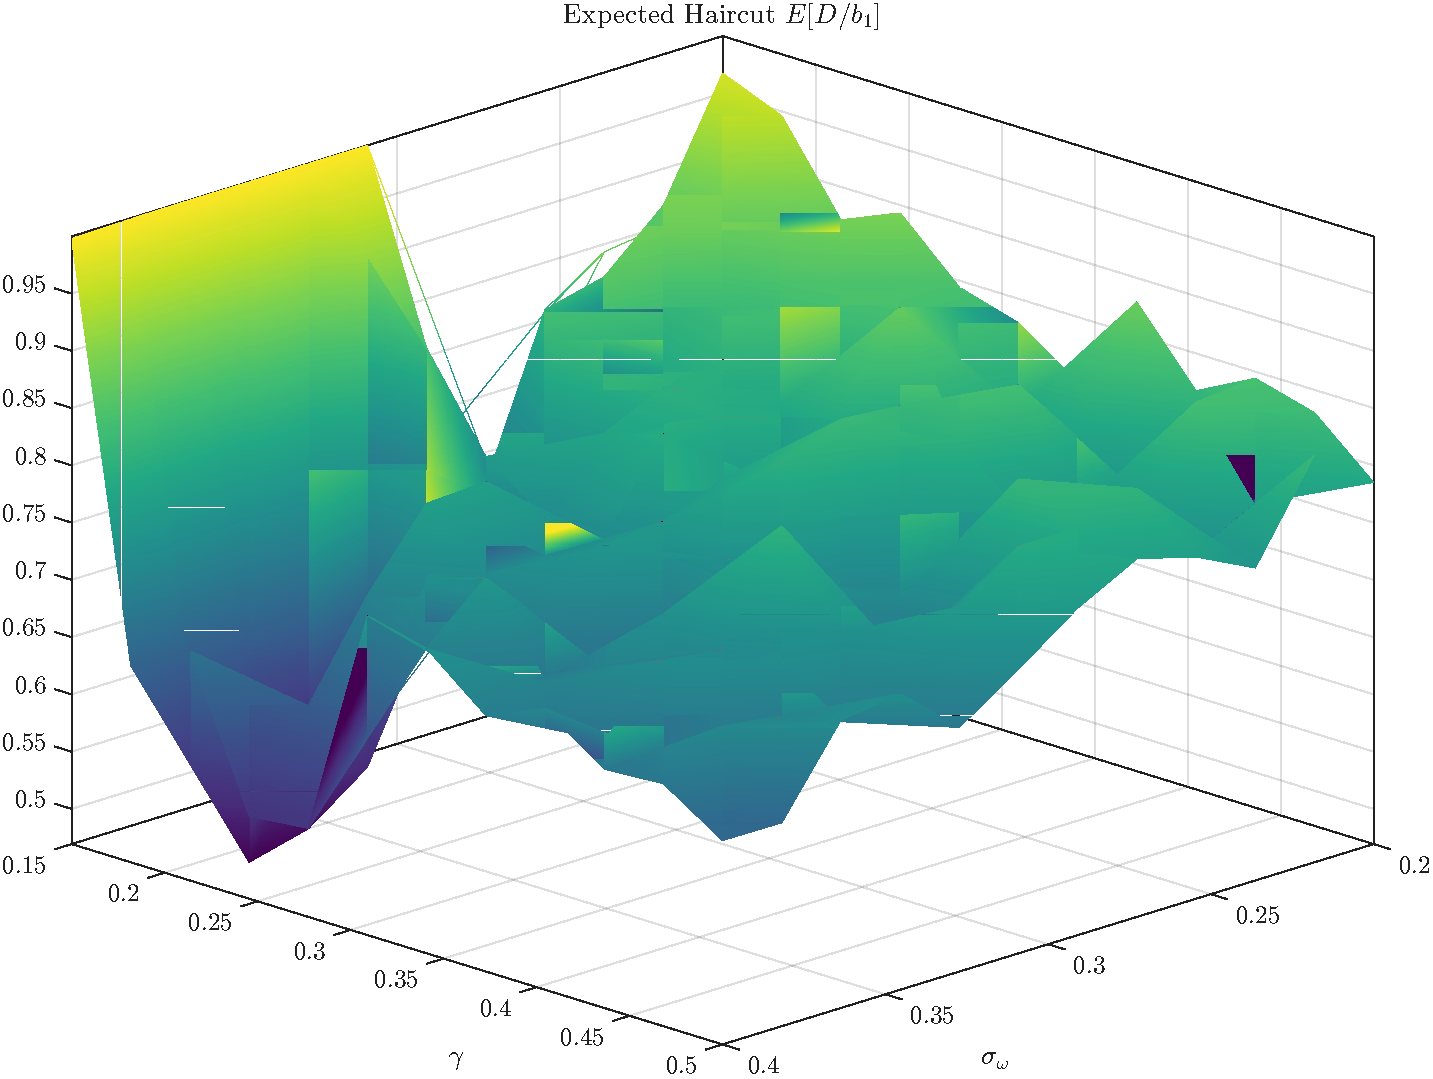
\includegraphics[width=0.8\linewidth]{cs_haircut.pdf}
    \caption{Haircut comparative static surface over $\gamma$ and $\sigma_{\omega}$, in general equilibrium under baseline calibration documented in Section \ref{sec:quantitative}.}
    \label{fig:cs_haircuts}
\end{figure}

\subsection{The Role of Idiosyncratic Banking Risk}\label{sec:comp_stat_sigma_omega}

The idiosyncratic productivity shock variance $\sigma_\omega^2$ is the primitive driver of financial fragility in this model. Following \citet{christiano_risk_2014}, who establish that variations in the cross-sectional standard deviation of idiosyncratic productivity (the ``risk shock") are the dominant driver of business-cycle fluctuations in financial variables, $\sigma_\omega$ feeds through to all key equilibrium objects of the model: the financial-friction wedge $\Psi(\bar\omega) \equiv \Gamma(\bar\omega) - \mu G(\bar\omega)$, the default threshold $\bar\omega$, the external finance premium $Z/R^*$, the import price $p_{m,1}$, and ultimately the household's optimal default policy $D(y_1, b_1)$.

The partial effects of $\sigma_\omega$ on the primitive CSV objects, at fixed $\bar\omega$, fall naturally from the log-normal specification (\ref{eq:omega_dist}), where an increase in $\sigma_\omega$ constitutes a mean-preserving spread of the idiosyncratic shock distribution:

\begin{enumerate}
    \item[(i)] $\partial \Gamma(\bar\omega) / \partial \sigma_\omega < 0$. The lender's expected revenue share falls: a wider distribution shifts mass into the default region $\omega < \bar\omega$ where the lender no longer collects $\bar\omega \cdot p_{m,t} m^f$ in full, and into the upper tail where the intermediary retains the residual surplus.
    \item[(ii)] $\partial (\mu G(\bar\omega)) / \partial \sigma_\omega > 0$. Expected auditing costs rise, as more probability mass falls below $\bar\omega$ and triggers the deadweight monitoring loss.
    \item[(iii)] $\partial \Psi(\bar\omega) / \partial \sigma_\omega = \partial \Gamma / \partial \sigma_\omega - \partial(\mu G) / \partial \sigma_\omega < 0$. The net surplus accruing to the lender per unit of intermediated imports unambiguously falls.
\end{enumerate}

From (\ref{eq:pm}), it is visible that, via result (iii), increases in $\sigma_{\omega}$ raises $p_{m,1}$ for any given leverage. Of more interest, the convexity of the import-price response in $D$, captured by the $\Psi(\bar\omega)^2$ denominator in (\ref{eq:dpm_dn}), intensifies in $\sigma_\omega$: as $\Psi$ shrinks, the same haircut produces a sharper net-worth-to-import-price pass-through. Idiosyncratic banking risk, in addition to shifting the equilibrium, increases curvature of the household's marginal cost-curve in default.

\begin{proposition}[Necessity of Idiosyncratic Banking Risk for Interior Default] \label{prop:internal_default}
Suppose $\sigma_{\omega}=0$, that is, that no idiosyncratic risk exists within the realised output of intermediated foreign goods supplied by domestic intermediaries. Then,
\begin{equation*}
    D^*=b_1 \quad \forall \quad b_1 \in [0,\infty),
\end{equation*}
in words, the household in equilibrium will optimally default on all issued debt, in all states, regardless of period 0 issuance. Therefore, for an interior default solution to be sustained in equilibrium it must be that $\sigma_\omega>0$. 

\noindent Proof: See Appendix~\ref{ap:internal_default_proof}.
\end{proposition}

\begin{figure}[!tbp]
  \centering
  \subfloat[EFP]{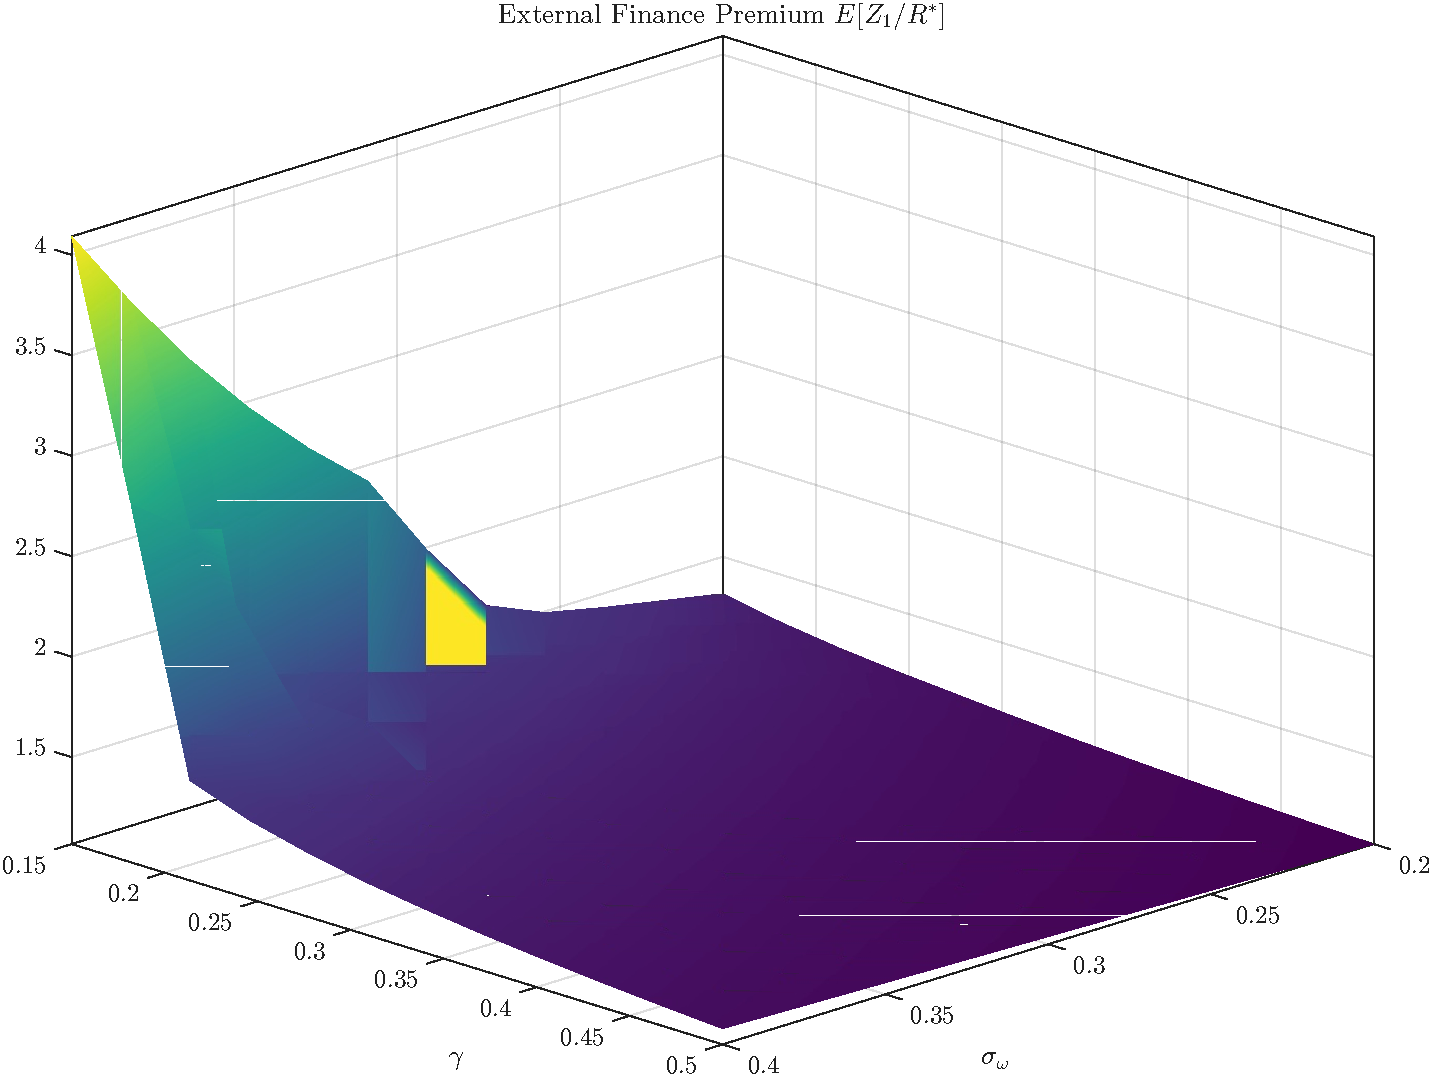
\includegraphics[width=0.8\textwidth]{cs_efp.pdf}}
  \hfill
  \subfloat[Import Compression]{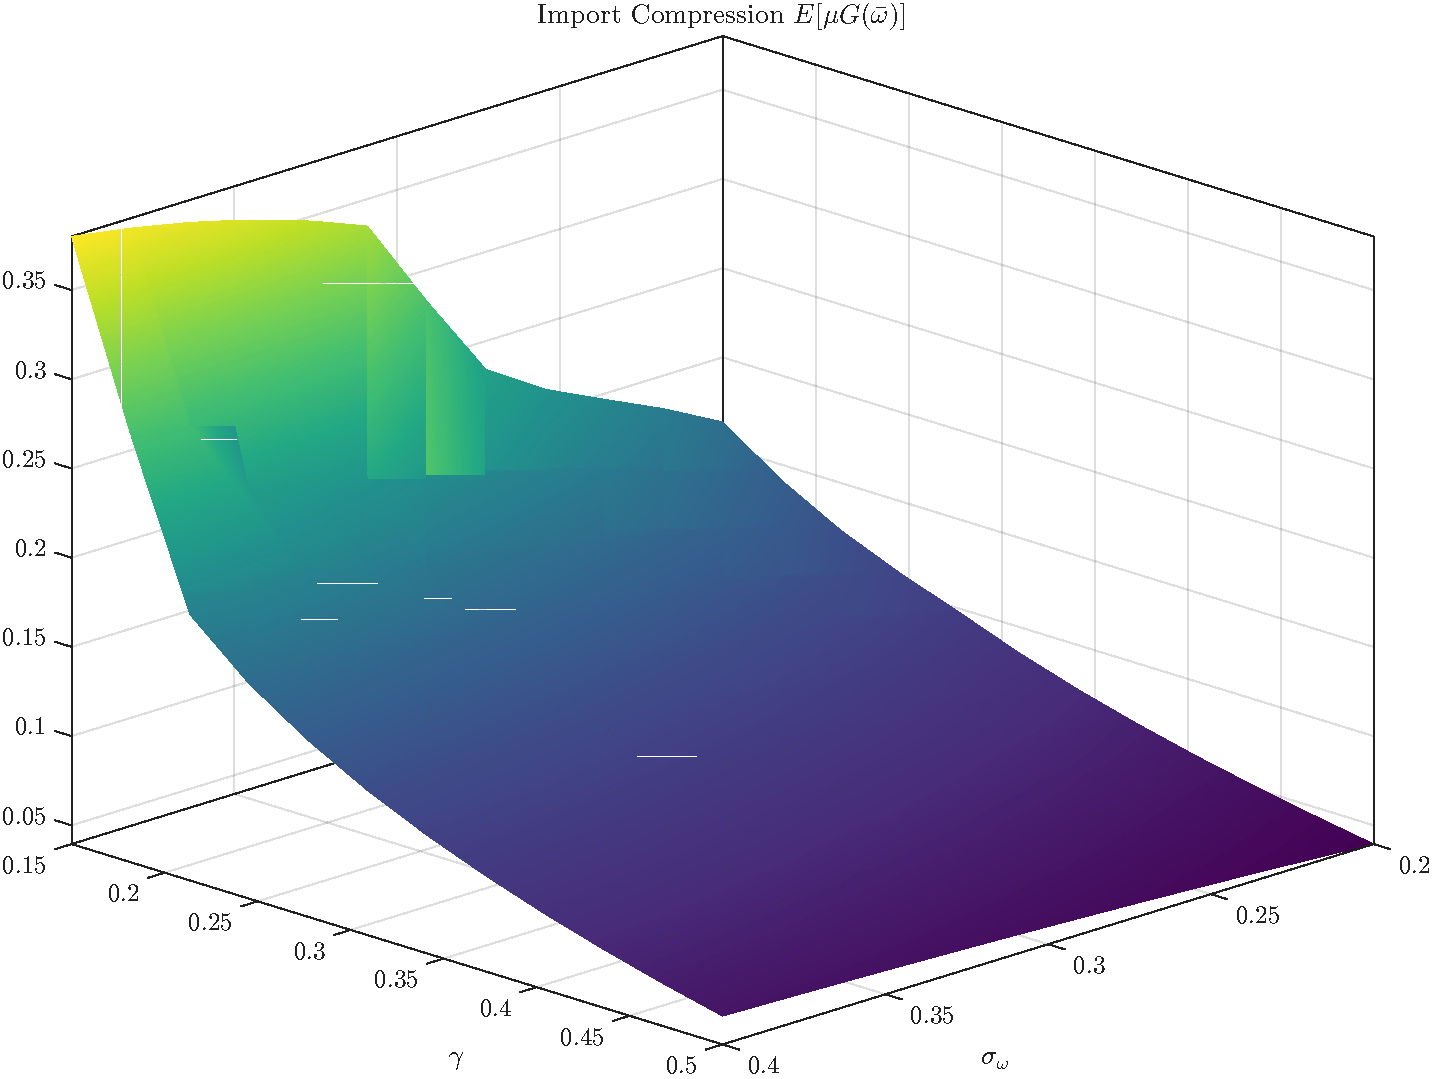
\includegraphics[width=0.8\textwidth]{cs_import_comp.pdf}}
  \caption{Financial comparative static surfaces over $\gamma$ and $\sigma_{\omega}$, in general equilibrium under baseline calibration documented in Section \ref{sec:quantitative}.}\label{fig:comp-stat-efp-imports}
\end{figure}

Herein the dialectical role banking risk has on sovereign default can be seen within this thesis; from Proposition \ref{prop:internal_default}, the presence of idiosyncratic risk within the banking sector is necessary to admit partial default in equilibrium. Conditional on this equilibrium, idiosyncratic risk acts as an exogenous commitment device for the household, increasing the marginal cost of defaulting, thus the expected haircut is \textit{lower} under an increased $\sigma_{\omega}$. Banking risk both gives rise to the continuous-default mechanism that is the central object of equilibrium allocations, and disciplines its severity at the margin. Figure~\ref{fig:comp-stat-efp-imports} reports the general equilibrium values of the external finance premium and import compression, offering quantitative confirmation of the commitment-device nature that default costs possess; exhibiting monotone  visibly convex increases in $\sigma_{\omega}$ and $1-\gamma$. The figure also illustrates the relatively greater sensitivity equilibrium allocations have to $\gamma$ over $\sigma_{\omega}$ within the calibrated parameter range.

\subsection{Welfare in Borrowing}

\paragraph{The Constrained Planner's Problem}\label{sec:planner}

Consider a domestic Ramsey planner who chooses $b_1$ in Period~0 to maximise household welfare, subject to the same Period~1 equilibrium conditions as the competitive economy. That is, the planner takes as given the Period~1 default rule $D(y_1, b_1)$ and the associated competitive equilibrium mappings for $(\bar{\omega}_1, M^f_1, p_{m,1}, C_1)$, but internalises the bond price schedule.
The planner solves:
\begin{equation}\label{eq:planner}
    \max_{b_1 \geq 0} \; u\!\bigl(C_0(b_1)\bigr) + \beta\,\E_0\!\bigl[u\!\bigl(C_1(y_1, b_1)\bigr)\bigr],
\end{equation}
\[
    m^d_0 = y_0 - b_0 + q_0(b_1)\cdot b_1 + \Pi_0.
\]

\begin{definition}[Constrained Planner's Equilibrium]\label{def:planner_equil}
    A constrained planner's equilibrium is an allocation $\{b_1^{P}, q_0^{P}, D^{P}(y_1)\}$ and associated prices and quantities such that:
    \begin{enumerate}[label=(\roman*)]
        \item $b_1^{P}$ solves the planner's problem \eqref{eq:planner};
        \item For each realisation $y_1$, the Period~1 equilibrium $(D, \bar{\omega}_1, M^f_1)$ satisfies the same system \eqref{eq:sys_leverage}--\eqref{eq:sys_default} as under the competitive equilibrium;
        \item The bond price satisfies the \textit{schedule} \eqref{eq:bondprice}.
    \end{enumerate}
\end{definition}

Whilst the planner's problem is identical to that of the atomistic household in Period 1, the critical distinction from the competitive equilibrium is that the planner perceives the total revenue from bond issuance as
\[
    \mathcal{R}(b_1) \equiv q_0(b_1)\cdot b_1,
\]
and therefore the marginal revenue from issuing an additional unit of debt is
\begin{equation}\label{eq:marginal_revenue}
    \mathcal{R}'(b_1) = q_0(b_1) + q_0'(b_1)\cdot b_1,
\end{equation}
where the competitive household perceives only the first term. The second term, $q_0'(b_1)\cdot b_1$, captures the debt-dilution externality, where additional borrowing raises expected default, depresses the bond price, and erodes the revenue raised on outstanding issuance.


\paragraph{The Welfare Wedge}\label{sec:wedge}

\begin{corollary}[Overborrowing under CSV-Constrained Partial Default]\label{prop:overborrowing}
Let $(b_1^{CE}, D^{CE})$ denote the competitive equilibrium allocation of Definition~\ref{def:equil} and $(b_1^{P}, D^{P})$ the constrained planner's allocation of Definition~\ref{def:planner_equil}. Suppose the equilibrium features interior partial default, $D \in (0, b_1)$, as guaranteed by Assumption~\ref{ass:interior}. Then
\[
    b_1^{CE} > b_1^{P}:
\]
the competitive household over-borrows relative to the constrained planner's optimum.
\end{corollary}

\begin{proof}
Differentiating the planner's objective \eqref{eq:planner} with respect to $b_1$ yields the first-order condition
\begin{equation}\label{eq:planner_foc}
    \lambda_0^{P}\,\mathcal{R}'(b_1) = \beta\,\E_0\!\left[\lambda_1\!\left(1 + \gamma\,m^f_1\,\frac{\partial p_{m,1}}{\partial N_1}\right) + u'(C_1)\,\frac{\partial C_1}{\partial D}\,\frac{\partial D}{\partial b_1}\right],
\end{equation}
where $\lambda_t$ is the shadow value of income \eqref{eq:shadow} and $\mathcal{R}(b_1) \equiv q_0(b_1)\,b_1$ is total bond revenue, so that $\mathcal{R}'(b_1) = q_0(b_1) + q_0'(b_1)\,b_1$. The competitive household's Euler equation \eqref{eq:euler} satisfies
\[
    \lambda_0\,q_0 = \beta\,\E_0\!\left[\lambda_1\!\left(1 + \gamma\,m^f_1\,\frac{\partial p_{m,1}}{\partial N_1}\right)\right].
\]
Evaluating \eqref{eq:planner_foc} at the competitive allocation (so that $\lambda_0^{P} = \lambda_0$) and subtracting the Euler equation identifies the welfare wedge
\begin{equation}\label{eq:wedge}
    \underbrace{\lambda_0\,q_0'(b_1)\cdot b_1}_{\text{debt-dilution externality}} - \beta\,\E_0\!\left[\underbrace{u'(C_1)\,\frac{\partial C_1}{\partial D}\,\frac{\partial D}{\partial b_1}}_{\text{insurance value of default}}\right].
\end{equation}
At any interior partial-default solution, the household's first-order condition \eqref{eq:foc_D} implies $\partial C_1/\partial D = 0$, so the insurance term vanishes and \eqref{eq:wedge} reduces to its first component. Since higher debt raises expected default and depresses the bond price, $q_0'(b_1) < 0$, the wedge is strictly negative. The planner therefore values an additional unit of $b_1$ strictly less than the competitive household at the competitive allocation, and so optimally chooses $b_1^{P} < b_1^{CE}$. \\
\end{proof}

\begin{remark}\label{rem:corner}
It is worth noting that this does not necessarily hold in corner solutions: the envelope condition from \eqref{eq:foc_D} does not bind, and the sign of the second term of \eqref{eq:wedge}, and thus the direction of borrowing compared to the planner's optimum depends on the magnitude of the CSV friction relative to the intermediary net-worth.\\
\end{remark}

The wedge \eqref{eq:wedge} admits a natural interpretation. Partial default, under incomplete markets, can be thought of as expanding the effective asset span of the non-contingent bond. With partial default, the household can smooth its state-contingent repayment, making the non-contingent bond behave more like a portfolio of Arrow securities. The more responsive $D(y_1,b_1)$ is to the state, the better the insurance properties of the debt instrument. Under the CSV friction, however, households are subject to a convex cost associated with this insurance and at an interior optimum the household equates the marginal benefit and marginal cost so that the insurance collapses and isolates the debt-dilution externality as the sole source of the wedge. The result is over-borrowing. However, with a large enough risk-shock, there is no restriction on the magnitude of this term; the insurance term can dominate the debt-dilution externality, flipping the sign of the wedge and rationalising \textit{under-borrowing} relative to the planner.

%========================================================================
\section{Quantitative Analysis} \label{sec:quantitative}
%========================================================================


I now move to examine the quantitative implications of the model by conducting numerical simulations. I have chosen to use Sri Lanka's 2021-2022 default period as a calibration anchor. Sri Lanka's recent and well-documented renegotiation with bilateral and multilateral creditors makes their default a prime candidate to simulate via a partial-default model. That being said, moment-matching within a two-period setting is less credible than in an infinite-horizon case; the absence of an ergodic distribution over debt and default outcomes means empirical moments such as average spreads, default frequency, and debt-to-GDP ratios cannot be targeted directly, and default costs cannot be spread onto a recursive continuation value. Rather, the quantitative analysis here serves the purposes of (i) demonstrating that the model admits a computable equilibrium with empirically reasonable values (ii) numerical demonstrations of the types of key comparative statics that would otherwise be challenging to derive analytically.

Under the model's two-period setting, each period is set to a length of five years. This setting seeks to strike a balance between temporal realism and calibration feasibility. Periods shorter than this length do not allow for a realistic time frame one would reasonably expect sovereign renegotiation to occur within. Five years allows Period 1 to capture equilibrium following complete conclusion of refinancing. On the other hand, longer period settings would lead to issues of liquidity in our chosen instrument of calibration - CDS Swaps. 5 year sovereign bond CDS contracts are generally more widely traded than 10 year, ensuring implied default probability is adequately captured in price data. Thus, the discount rate and risk-free rate are calibrated to their respective five year compounded values. For the remainder of the quantitative analysis, I set my utility function to a CRRA arrangement,
\begin{equation*}
    u(C_t)=\frac{C_t^{1-\sigma_u}}{1-\sigma_u},
\end{equation*}
where $\sigma_u$ is the coefficient of relative risk aversion.

The model is solved numerically through a nested optimisation architecture. The Period 0 equilibrium is recovered by maximising the household's lifetime value function over $b_1$, with the expectation approximated by a seven-node Gauss-Hermite quadrature. For each candidate $b_1$ and quadrature node $y_1$, the Period 1 equilibrium is solved for. $D^*(y_1, b_1)$ is found by maximising the household's Period 1 utility over $D \in [0, b_1]$. At each candidate $D$, the leverage-threshold condition (\ref{eq:omega_leverage}) is solved analytically for $M^f_1$ in terms of $\bar\omega_1$, leaving the foreign-input market-clearing condition (\ref{eq:mc_foreign}) as a single equation in $\bar\omega_1$ which is solved residually. The total derivative $\partial p_{m,1}/\partial N_1$ entering the Period 0 Euler equation is computed at the optimum $D^*$ via central finite differences on the inner solver.

\subsection{Baseline Calibration: The Case of Sri Lanka}

Leading up to Sri Lanka's 2021--22 default, government revenue in 2019 as a percentage of GDP fell from ~12\% to ~8\% following reductions to value-added and labour taxation. Fiscal deterioration worsened following the collapse of tourism receipts following COVID-19, and spikes in wheat and fuel prices induced by Russia's invasion of Ukraine. A ban on chemical fertiliser imports drove down agricultural yields in 2021, forcing greater food imports and leaving the economy particularly susceptible to a balance-of-payments crisis. Foreign exchange reserves fell by ~99\% from 2019--22, and public debt rose to well above 100 \% of GDP, characterising a \textit{twin-deficits} crisis. Sri Lanka declared a unilateral external debt moratorium on 12th of April 2022. As expected from Proposition~\ref{prop:convexity}, imports contracted significantly in the months following restructuring. Credit Default Swaps (CDS) on government bonds soared during this period (Figure \ref{fig:sri_cds}). Gross non-performing loan ratios also rose significantly from $4.7\%$ in 2019 to $13.3\%$ by the end of 2022, underscoring the reciprocal banking crisis accompanying the sovereign default that would be visible under pronounced idiosyncratic banking risk. Under these patterns exhibited during a protracted restructuring period, Sri Lanka is an insightful baseline to quantitatively map financial intermediation exposure to sovereign risk and real equilibrium costs.

\begin{figure}
    \centering
    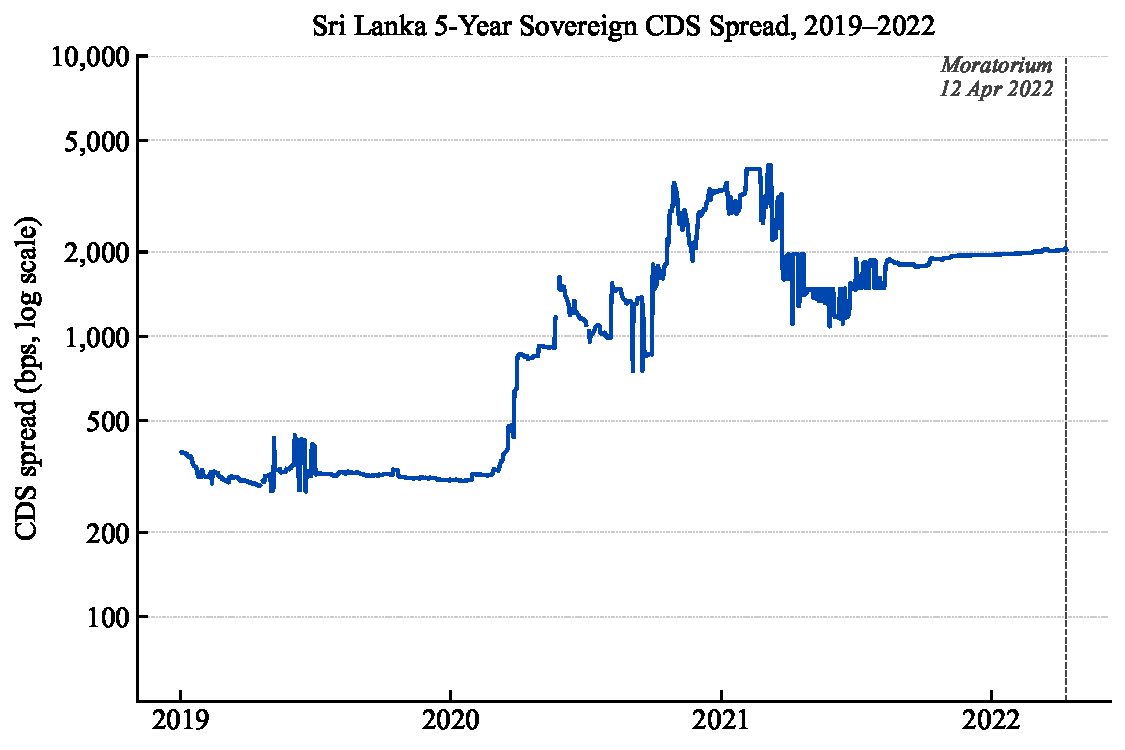
\includegraphics[width=1\linewidth]{sri_lanka_cds.pdf}
    \caption{Sri Lanka 5Y USD CDS spreads from 2019--2022. Source: Capital IQ.}
    \label{fig:sri_cds}
\end{figure}

\begin{table}[htbp]
    \centering
    \renewcommand{\arraystretch}{1.2}
    \resizebox{\textwidth}{!}{%
        \begin{tabular}{@{}ccccccccc@{}}
                \begin{tabular}{@{}lcll@{}}
                    \toprule
                    \textbf{Parameter} & \textbf{Value} & \textbf{Description} & \textbf{Source / Target} \\
                    \midrule
                    \multicolumn{4}{@{}l}{\textit{Preferences}} \\
                    $\beta$ & 0.815 & Subjective discount factor (5-year) & \\
                    $\sigma_u$ & 2.000 & Coefficient of relative risk aversion & \\
                    \addlinespace
                    
                    \multicolumn{4}{@{}l}{\textit{Technology and Trade}} \\
                    $\alpha$ & 0.700 & Armington weight on domestic inputs & Import share (World Bank)\\
                    $\eta$ & -1.000 & CES substitution parameter & \\ 
                    \addlinespace
                    
                    \multicolumn{4}{@{}l}{\textit{Financial Sector and Frictions}} \\
                    $\bar{n}_{base}$ & 0.065 & Long-run non-sovereign asset stock & CBSL Monetary Survey\\
                    $\gamma$ & 0.320 & Home bias share of sovereign debt & CBSL Monetary Survey \\
                    $\sigma_\omega$ & 0.250 & Idiosyncratic shock volatility & \citet{christiano_risk_2014} \\
                    $\mu$ & 0.400 & CSV monitoring / auditing cost & \citet{christiano_risk_2014} \\
                    \addlinespace
                    
                    \multicolumn{4}{@{}l}{\textit{International Market}} \\
                    $R^*$ & 1.104 & World gross risk-free interest rate & \\ 
                    \addlinespace
                    
                    \multicolumn{4}{@{}l}{\textit{Endowment and Debt Process}} \\
                    $y_0$ & 1.000 & Period 0 endowment & Normalisation \\
                    $b_0$ & 0.180 & Pre-existing debt (Implied debt-to-GDP) & CBSL Annual Report \\
                    $\rho$ & 0.600 & AR(1) persistence of endowment growth &  \\
                    $\mu_g$ & 1.200 & Unconditional mean growth rate & World Bank WDI (2015-2019 Avg) \\
                    $\sigma_g$ & 0.150 & Growth shock standard deviation & Scaled from \citet{arellano_default_2008} \\
                    \bottomrule
                \end{tabular}
        \end{tabular}
    }
    \caption{Baseline Parameterisation}
    \label{tab:calibration}
\end{table}

\subsubsection*{Calibration Strategy}

The model contains fourteen parameters. Preferences, the elasticity of substitution between domestic and foreign inputs, and the world risk-free rate are set externally, anchored to standard values in the quantitative sovereign default and emerging-market business cycle literatures. Financial sector parameters $(\bar{n}_{\mathrm{base}}, \gamma, \sigma_\omega, \mu)$ and the pre-existing debt stock $b_0$ are calibrated to Sri Lanka-specific data, primarily drawn from the Central Bank of Sri Lanka (CBSL) Monetary Survey and CBSL Annual Reports for the pre-crisis window 2017--2018.

I chose to anchor the calibration via the expected haircut, $\E\left[ {D}/{b_1}\right]$, in the model to target the implied expected loss backed out of credit-default swap data. Specifically, I look at Sri Lankan 5 year CDS pricing data, with implied default probability generated from the standard ISDA model with an assumed recovery rate of 40\%. Following Sri Lanka's sovereign default episode in 2021-22, the average daily implied default probability rose to $\approx 78\%$, from $\approx 22\%$ the prior five years. The resulting target is an expected loss of $\approx0.468$. This expected loss serves as the primary empirical moment targeted by the model's expected haircut. Table \ref{tab:calibration} documents the baseline calibration to Sri Lankan variables during this episode of default.

\paragraph{Preferences and Technology}

The annual subjective discount factor is set to $0.96$, the standard value in the quantitative sovereign default. Under the model's 5-year period formulation this is compounded as $\beta = 0.96^5 = 0.815$. The coefficient of relative risk aversion under the CRRA specification follows \citet{arellano_default_2008}, \citet{mendoza_general_2012}, and the broader \citet{eaton_debt_1981} literature. The CES weight on domestic inputs targets Sri Lanka's pre-crisis import share of GDP. The import share implied by the household's intratemporal optimum is
\[
  s_m \equiv \frac{R^* m^f_0}{m^d_0 + R^* m^f_0} 
  = \left[1 + \left(\frac{\alpha R^*}{1-\alpha}\right)^{\sigma} 
  R^{*\,-1}\right]^{-1}.
\]
The 2017--2018 average of Sri Lanka's imports of goods and services as a share of GDP pins down $s_m = 0.27$,
which with a $\sigma = 0.5$ results in a calibrated $\alpha \approx 0.7$. The CES Elasticity of substitution $\eta = -1$ parameter is set to maintain gross complementarity required for import compression to translate into consumption losses, and within the range used in the emerging-market open-economy literature \citep{mendoza_general_2012}.

\paragraph{Financial Sector and Frictions}

The annual world risk-free rate is set to $2\%$, loosely matching the 5-year US Treasury constant maturity yield 
averaged over 2017--2018 (Federal Reserve H.15). Compounded over five years, $R^* = (1.02)^5 = 1.104$.

Sri Lankan financial sector parameters are primarily based upon data published by the Central Bank of Sri Lanka (CBSL)\footnote{These statistics can be accessed within the \href{https://www.cbsl.gov.lk/en/publications/economic-and-financial-reports}{CBSL's Monetary Survey}.}. $\bar n$ here is calibrated to the average pre-crisis (2017--2018) equity capital held by licensed commercial banks (LCBs) as a share of nominal GDP. From the CBSL's Monetary Survey, Table 4.07, the \textit{Paid-up Capital, Reserve Fund and Undistributed Profits} as a percentage of nominal GDP averages to $\approx0.065$.

$\gamma$ is calibrated to the ratio of sovereign debt exposure of LCBs to total local-currency debt issued by the Government of Sri Lanka (net of central bank holdings),
\begin{equation*}
    \gamma=\frac{\text{LCB holdings of LKR govt securities}}{\text{Total outstanding LKR govt securities (net of CBSL holdings)}}
\end{equation*}
The local currency debt focus reflects that sovereign-bank nexus in Sri Lanka operates almost exclusively through the LKR debt market, with a negligible share of international sovereign bonds held by LCBs. From the CBSL Monetary Survey, Table 4.07, LCBs held an average of LKR 1,453,360 million in Government of Sri Lanka Obligations between 2017--2018, whereas the total outstanding local debt average in the same period equals LKR 5,109,460 million, from the CBSL's \textit{Public Debt Management
in Sri Lanka} 2018 report, under \textit{Key Government Debt Indicators}\footnote{Report available published by the \href{https://www.cbsl.gov.lk/sites/default/files/cbslweb_documents/publications/otherpub/public_debt_management_in_sri_lanka_2018.pdf}{ CBSL}.}. These figures result in a calibrated $\gamma\approx 0.25$.

CSV auditing parameter $\mu$ follows standard \citet{bernanke_chapter_1999} style calibrations, sitting slightly above the high-end of \citet{carlstrom_agency_1997}'s estimates, reflecting Sri-Lanka's weaker bankruptcy infrastructure\footnote{The World Bank's \textit{Doing Business} ``Resolving Insolvency" indicator places Sri Lanka as 94th of 190 in 2020 \citep{world_bank_doing_2020}. Most relevant to my calibration, the recovery rate for secured creditors is listed as 0.43 cents on the dollar, mapping to auditing costs of 0.57. I split the difference between this rate and the estimates of \citet{carlstrom_agency_1997} in my calibration of $\mu=0.46$.}.
The idiosyncratic intermediary productivity shock governs the curvature of the CSV friction, and through it the convexity of the default penalty (Proposition~\ref{prop:convexity}). The baseline business-cycle calibration of 
\citet{christiano_risk_2014} uses $\sigma_\omega \approx 0.26$ in non-crisis periods, but their estimated time-series (Figure 7) shows pronounced spikes in $\sigma_\omega$ during financial-distress, with peak values exceeding $0.4$ in recessions. Since the model is calibrated to a twin-deficits crisis period with sharply deteriorating LCB asset quality, I anchor $\sigma_\omega$ to the upper region of the \citet{christiano_risk_2014} estimated range, $\sigma_\omega = 0.40$.

\paragraph{Endowment and Debt Process}

The stock of pre-existing external debt obligations, expressed as a share of Period~0 endowment ($b_0=0.180$), targets Sri Lanka's 
total cumulative repayment burden over the 5 year pre-crisis period. The external debt service between 2017--2018 averages around 4\% to 5\% of GDP, which cumulated over 5 years $\approx20\%-25\%$. The baseline calibration targets the lower end of this range. The growth processes persistence $\rho=0.05$ broadly targets emerging market estimates from Table 2 within \citet{aguiar_emerging_2007}, which compounded to the 5 year period formulation implies that every 5 year window essentially acts as an independent draw, with previous shocks failing to persist into the next period. Sri Lanka's mean annual real GDP growth over 2015--2019 is $\approx 3.7\%$, giving $\mu_g = (1.037)^5 \approx 1.20$. The Period~0 conditioning state for the growth process is set at $0.95$, approximately targeting Sri Lanka's 3.6\% real GDP contraction in 2020. The growth-shock standard deviation $\sigma_g$ is scaled from \citet{aguiar_emerging_2007}, who estimates an annual standard deviation of $\approx 0.028$ for emerging-market trend-growth innovations. Under the calibrated $\rho \approx 0$, this target aggregates as $\sigma_g \approx 0.028 × \sqrt5 \approx 0.063$. The baseline $\sigma_g = 0.150$ sits marginally above this benchmark range to ensure the seven-node Gauss-Hermite support spans both crisis and near-repayment states with sufficient probability.

\begin{table}[htbp]
    \centering
    \renewcommand{\arraystretch}{1.2}
    \renewcommand{\thefootnote}{\fnsymbol{footnote}} 
    
    \begin{tabular}{@{}lrlr@{}}
        \toprule
        \multicolumn{2}{@{}l}{\textbf{Period 0 Allocations}} & \multicolumn{2}{l@{}}{\textbf{Expected Period 1 Outcomes}} \\
        \midrule
        Consumption ($C_0$)         & 0.8378 & Expected Default ($\E[D]$)            & 0.2348 \\
        Domestic Goods ($m_{d,0}$)  & 0.9899 & Expected Haircut ($\E[D/b_1]$)        & 0.5558 \\
        Imported Goods ($m_{f,0}$)  & 0.6168 & Expected Recovery ($\E[1 - D/b_1]$)   & 0.4442 \\
        Debt Issued ($b_1$)         & 0.4223 & Expected Consumption ($\E[C_1]$)      & 0.5110 \\
        Bond Price ($q_0$)          & 0.4023 &                                       &        \\
        Spread (bps, annualised)\footnotemark[1] & 2{,}038 &                         &        \\
        \bottomrule
    \end{tabular}
    \caption{Period 0 Equilibrium and Expected Macroeconomic Moments.}
    \label{tab:period0_summary}
\end{table}

% Wrap the footnotetext in a group to strictly enforce the symbol
\begingroup
\renewcommand{\thefootnote}{\fnsymbol{footnote}}
\footnotetext[1]{Under the two-period model formulation where each period corresponds to five years, the cumulative spread is converted to an annualised basis-point measure via $\text{spread}_{\text{ann.}} = \left[(R^*/q_0)^{1/5} - (R^*)^{1/5}\right] \times 10{,}000$.}
\endgroup

\subsubsection*{Baseline Results}

The baseline calibration results, reported in Tables \ref{tab:period0_summary} and \ref{tab:period1_states}, shows a generated haircut marginally above the targeted CDS-implied expected loss by $\approx 10 \text{ percentage points}$, though within range of a highly distressed default and credit environment, consistent with the 2021--22 period in Sri Lanka. Likewise, the annualised spread generated broadly targets peak Sri Lanka 5 Years USD / United States 5 Years Government Bond Spread in 2022 of $\approx 2500\text{ bps}$, undershooting by around 460 points. \\

\begin{table}[htbp]
    \centering
    \renewcommand{\arraystretch}{1.2}
    \small
    \resizebox{\textwidth}{!}{%
        \begin{tabular}{@{}ccccccccc@{}}
            \toprule
            \textbf{Endowment} & \textbf{Default} & \textbf{Haircut} & \textbf{Bank Default} & \textbf{Bank} & \textbf{Import} & \textbf{Imports} & \textbf{Consumption} & \textbf{Finance} \\
            \textbf{Shock} & \textbf{Level} & \textbf{Fraction} & \textbf{Threshold} & \textbf{Assets} & \textbf{Price} & & & \textbf{Premium} \\
            $y_1$ & $D$ & $D/b_1$ & $\bar{\omega}_1$ & $M^f_1$ & $p_{m,1}$ & $m_{f,1}$ & $C_1$ & $Z/R^*$ \\
            \midrule
            0.5943 & 0.3582 & 0.8482 & 0.6744 & 0.2422 & 1.1164 & 0.2292 & 0.3123 & 1.1380 \\
            0.7314 & 0.3215 & 0.7612 & 0.6744 & 0.2881 & 1.1164 & 0.2725 & 0.3715 & 1.1380 \\
            0.8772 & 0.2824 & 0.6686 & 0.6744 & 0.3369 & 1.1164 & 0.3187 & 0.4344 & 1.1380 \\
            1.0431 & 0.2379 & 0.5633 & 0.6744 & 0.3923 & 1.1164 & 0.3712 & 0.5059 & 1.1380 \\
            1.2403 & 0.1851 & 0.4382 & 0.6744 & 0.4583 & 1.1164 & 0.4336 & 0.5909 & 1.1380 \\
            1.4876 & 0.1188 & 0.2812 & 0.6744 & 0.5410 & 1.1164 & 0.5118 & 0.6976 & 1.1380 \\
            1.8307 & 0.0268 & 0.0634 & 0.6744 & 0.6558 & 1.1164 & 0.6204 & 0.8456 & 1.1380 \\
            \bottomrule
        \end{tabular}
    }
    \caption{State-Contingent Equilibrium Outcomes in Period 1}
    \label{tab:period1_states}
\end{table}

The model exhibits default that is strongly state-contingent. Haircut severity falls monotonically with the realised endowment: the sovereign defaults most in low-output states and least in high-output states. Of note, the default policy does not reach a full-default corner in the worst endowment state and approaches a low-haircut repayment region in the best state. Under the baseline calibration, allocations span both crisis and near-repayment states within the same default policy.

Interestingly, when in an interior-default state, the sovereign adjusts its haircut to endogenously target a particular default threshold, holding import prices and external finance premiums close to a common level across states. This is a numerical consequence of the household's default policy (\ref{eq:KT}): the sovereign chooses the haircut until the marginal budgetary gain from default equals the marginal import-price cost. Whilst not listed in Table 3, states where an upper corner solution is reached produce a lower finance premium, a consequence of the marginal benefit of defaulting exceeding the marginal cost.

Finally, the baseline simulation illustrates that larger haircuts do indeed generate  greater import compression, lowering consumption in kind. Convexity in import compression cannot be assessed here, as these equilibrium allocations are non-conditional in haircut size. For conditional analysis of import compression, see Figure \ref{fig:comp-stat-efp-imports}.

\subsection{Benchmark Decomposition without Banking Sector} \label{sec:mech_decomp}

In previous sections I have documented the analytical claim for necessity of $\mu$, in Remark 1, and $\gamma$, in Section~\ref{sec:optimality}, for structural convexity in the default penalty and import compression. Here, under the baseline calibration documented above, I illustrate such necessity claims numerically by solving for equilibrium outcomes under the limiting cases of $(\gamma, \mu) \to 0$.

\paragraph{$\mu=0$ shut-off}

Equilibrium allocation comparisons under the limiting case of $\mu=0$ with baseline are reported in Table~\ref{tab:mu_shutoff}. Under the shut-off case, the threshold $\bar \omega$ is dramatically raised out of the operating region of Assumption~\ref{ass:operating_region}, causing significant state-regions of total default. The cost of default is now so low that the marginal benefit (almost) always exceeds the marginal cost. Imports become insensitive to the haircut $\partial p_{m,1}/\partial D\approx0$, and convexity of default costs are shut down. This illustrates the necessity of the CSV friction for convex graded imports in haircut size. The bond price collapses, entering a no-trade region (Assumption~\ref{ass:interior}). This is mechanistically comparable to the removal of bailouts in \citet{hur_optimal_2021}, with the reverse consequences for default cost magnitude.

\begin{table}[ht]
\centering
\begin{tabular}{lcc}
\toprule
& Baseline ($\mu = 0.46$) & Shut-off ($\mu = 0$) \\
\midrule
Expected haircut $\mathbb{E}[D/b_1]$       & 0.556 & 0.907 \\
Upper-corner states (out of 7)              & 0     & 3     \\
Bond price $q_0$                            & 0.402 & 0.084 \\
Equilibrium threshold $\bar\omega^*$        & 0.674 & $\approx 5$ (upper tail)$^\dagger$ \\
$p_{m,1}$  &   1.116    &   1.009 \\
\bottomrule
\end{tabular}
\caption{Equilibrium moments under the CSV friction shut-off. $^\dagger$The precise value of $\bar\omega^*$ in the upper-tail regime is solver-sensitive because $\Gamma'(\bar\omega) \to 0$ renders the leverage-threshold condition \eqref{eq:omega_leverage} near-degenerate.}
\label{tab:mu_shutoff}
\end{table}

\paragraph{$\gamma=0$ shut-off}

The equilibrium results comparisons with baseline under $\gamma\to 0$ are reported in Table~\ref{tab:gamma_shutoff}. Following the comparative static-based analysis written in Section~\ref{sec:comp_stat_gamma}, it is visible that the severing of the net-worth channel induces a no-trade equilibrium mechanically, admitting zero issuance from the household, as the lender prices in a probability of default $=1$. The bank-exposure channel is therefore necessary for partial sovereign default to obtain in equilibrium, mirroring the role of idiosyncratic risk in Proposition~\ref{prop:internal_default}.

\begin{table}[ht]
\centering
\begin{tabular}{lcc}
\toprule
& Baseline ($\gamma = 0.25$) & Shut-off ($\gamma = 0$) \\
\midrule
Equilibrium debt issuance $b_1^*$       & 0.4223 & 0 \\
Bond price $q_0$                         & 0.4023 & 0 \\
Expected haircut $\mathbb{E}[D/b_1]$     & 0.5558 & undefined \\
Period 0 consumption $C_0$               & 0.838  & 0.694 \\
\bottomrule
\end{tabular}
\caption{Equilibrium moments under the bank-exposure shut-off. To preserve balance-sheet size invariance $\bar{n}$ is adjusted to $\bar{A} = 0.1226$ when $\gamma = 0$.}
\label{tab:gamma_shutoff}
\end{table}

Combining these two shut-off results illustrates a key necessity characteristic underlying the framework's endogenous import-haircut contribution. The two structural primitives of the financial-intermediation channel, bank exposure $\gamma$ and the CSV auditing friction $\mu$, are jointly necessary for the mechanism: $\gamma$ for its existence, and $\mu$ for its convexity.


%========================================================================
\section{Discussion} \label{sec:discussion}
%========================================================================

\subsection{Testable Predictions}\label{sec:predictions}

The comparative statics of Section \ref{sec:implications} and analysis in Section \ref{sec:quantitative} admit a series of empirical predictions that can be taken to the data:

\paragraph{Prediction 1: Import compression is graded in haircut severity}
\emph{Across restructuring episodes, larger realised haircuts should be associated with larger contractions in imports, especially in economies where imported inputs are difficult to substitute with domestic production.} Whilst \citet{mendoza_general_2012} document the relationship between default and import-based financial frictions, the friction is still generated via a binary market-exclusion channel; here, I propose an endogenous channel where import compression rises continually, and nonlinearly, in haircut.

\paragraph{Prediction 2: The haircut-import elasticity is increasing in domestic bank sovereign exposure}
\emph{The elasticity of imports with respect to haircut severity is larger in countries with greater domestic bank exposure to sovereign debt.} The doom-loop literature \citep{sosa-padilla_sovereign_2018, brunnermeier_sovereign-bank_2016} establishes that sovereign distress propagates to the financial sector, but does not deliver a graded cross-sectional prediction tied to a structural exposure parameter. By isolating $\gamma$ as the share of sovereign losses transferred to intermediaries, the model proposed in this thesis generates a direct mapping from this exposure to the \textit{slope} of the haircut-import relationship.

\paragraph{Prediction 3: Output losses are convex in haircut severity}
\emph{The relationship between haircut severity and post-default output decline is nonlinear: larger haircuts are associated with disproportionately larger output losses. This convexity is stronger in economies with higher domestic bank exposure to sovereign debt.} The increase in the curvature of this relationship in domestic bank exposure to sovereign debt cannot be rationalised without the modeling combination of bank net-worth erosion and partial default.

\paragraph{Prediction 4: Haircuts increase monotonically and with convexity in debt-to-GDP} 
\emph{In a cross-section of sovereign restructuring episodes, realised haircuts are positively associated with the pre-default debt-to-GDP ratio.} This is a standard prediction rationalised by existing models of partial default \citep{arellano_partial_2023, goodhart_debt_2018, peiris_capital_2025}, and the model proposed in this thesis continues to generate this convex debt-to-GDP relationship with default.

\subsection{Limitations and Further Research}

% Weakness: always default, 
% Realistics spreads in quant analysis should be reserved to infinite-time horizon model
% If banks hold a small enough share of sovereign debt, the pass-through coefficient scales the marginal cost down. As γ→0, the marginal cost vanishes — but so does the *channel*: defaulting doesn't hurt you because banks don't hold the debt. In the limit γ=0 the model degenerates to one with no transmission, and the household defaults fully (since there's no cost).
% Also, reduced form
% Discussion of assumptions (1&2)

The most obvious direction for future research from the theoretical framework posed in this thesis is to extend the two-period model to an infinite-horizon setting. This would enable the model to speak to debt-accumulation dynamics, transition paths post-default (allowing exploration of serial-default) and more sophisticated moments-matched calibrations to a panel of emerging economies. The kinks at the corners of the household's default function under continuous partial default, combined with a large state-space including both $(b_t,N_t)$, generates a high computational cost associated with numerical solutions; this should not be prohibitive, however.

Assumption \ref{ass:interior} rules out the no-trade corner and ensures interior bond-market participation, which in turn delivers the continuous default severity that is the model's central object of analysis. In the calibrated equilibrium, however, the sovereign defaults in every state of nature, with severity varying from near-full default in the worst endowment state to a low haircut in the best. Empirically, this is at odds with observed default frequencies in emerging-market panels, and as such the model speaks only to the intensive margin of default rather than to the extensive margin of \textit{when} default occurs. This is not a limitation of Assumption 1 in isolation: in an infinite-horizon extension, the continuation value would likely discipline the default decision sufficiently to generate repayment regions in sufficiently good states. In the two-period setting, the assumption binds more tightly than it would otherwise.

An infinite-horizon extension would also allow for the opportunity to discipline banking parameters $\gamma,\bar{n}$, which the equilibrium allocations are highly sensitive to, by using richer micro-level data. $\gamma$ in particular is reduced-form by construction and acts as a key structural parameter - endogenising intermediary portfolio choices, following \citet{farhi_deadly_2018} for example, may provide richer equilibrium dynamics by removing a free parameter. Whilst $\gamma$ is well-interpretable as the portfolio-adjustment towards or away from domestic sovereign debt, generated by home-bias or financial repression, the parameter loses this interpretation when set to zero; the household is no longer subject to the intermediary-mediated default penalty. Examination of default induced by the \textit{existence} of idiosyncratic risk, rather than sensitivity to risk, would necessitate reworking of this parameter. Finally, the cash-in-advance nominal set-up delivers nominal neutrality (Lemma \ref{lem:neutrality}) by construction; introducing nominal rigidities would fundamentally change the implications of the CSV transmission mechanism, and would allow for analysis of real exchange rate dynamics, following the work of \citet{na_twin_2018}.

\subsection{Conclusion}

This thesis proposed a general equilibrium model for studying how the severity of haircuts transmits to import prices and household consumption, amplified by domestic financial intermediation. Partial sovereign default raises the strength and convexity of import compression through two distinct margins of the financial friction. On the one hand, domestic banks exposed to sovereign debt see their balance sheets erode in default, raising the external finance premium charged on working capital and the price at which imports are intermediated. On the other hand, idiosyncratic risk in import intermediation produces a costly-state-verification friction that increases in convexity as intermediary net worth falls, generating a marginal cost of default that grows disproportionately in haircut severity. The calibration of the model to Sri Lanka's 2021--22 default episode indicates that both mechanisms operated at empirically reasonable magnitudes during the crisis.

The partial default framework posed in this paper provides a unique quantitative tool for generating an intensive, graded structural mapping between empirically observable sovereign debt exposure in the domestic banking sector and the level of import compression post-restructuring. The cross-country empirical predictions admitted by the model invite investigation via an extended panel of restructuring episodes, representing an opportunity for future work.

%========================================================================
\newpage
\printbibliography
\newpage
%========================================================================

\begin{appendices}

\section{Nominal Structure and Exchange Rate} \label{ap:nominal}
Let $P_t$ denote the domestic-currency price of domestic goods, and $e_t$ the exchange rate, expressed as units of domestic currency per unit of foreign currency. The real exchange rate is defined as
\begin{equation} \label{eq:real-exch}
    RER_t \equiv \frac{e_t}{P_t},
\end{equation}
where foreign input prices are normalised to one. I assume that bonds within the domestic economy are issued in real-terms, representing a fixed quantity of domestic output, as to ensure the real net-of-default payoff for the household is invariant to domestic price levels. \\

Domestic input purchases are subject to a cash-in-advance constraint that pins down domestic price levels:
\begin{equation} \label{eq:cash-in-advance}
    MS_t=P_t \cdot m^d_t,
\end{equation}
where $MS_t$ denotes the domestic money supply. The lack of nominal rigidities here allows recovery of the nominal neutrality result of Lemma \ref{lem:neutrality}.

\begin{lemma}[Nominal Neutrality]\label{lem:neutrality}
Suppose that:
\begin{enumerate}[label=(\roman*)]
    \item sovereign bonds are denominated in units of the domestic good, so that the real payoff $(b_1 - D)$ is independent of $P_t$;
    \item domestic goods prices are fully flexible; and
    \item the real exchange rate is constant: $RER_t = \bar{RER}$ for all $t$.
\end{enumerate}
Then the real allocation $\{C_t,\, m^d_t,\, m^f_t,\, M^f_t,\, b_1,\, D,\, \bar{\omega}_t,\, Z_t,\, \Pi_t\}_{t=0,1}$ and the real prices \\
$\{q_0,\, p_{m,0},\, p_{m,1}\}$ are determined by the system of equations \emph{\eqref{eq:CES}}--\emph{\eqref{eq:euler}}  independently of the domestic money supply $MS_t$, the nominal exchange rate $e_t$, and the domestic price level $P_t$. The nominal variables are determined residually by:
\begin{equation}\label{eq:price-level}
    P_t = \frac{MS_t}{m^d_t}, \qquad e_t = P_t \cdot \bar{RER},
\end{equation}
where $\bar{RER} = 1$.

\end{lemma}

\begin{proof} \label{proof:neutrality}
\textit{of Lemma \ref{lem:neutrality}} Express each agent's budget constraint and optimality condition in nominal terms, then deflate by $P_t$. The household's Period 1 nominal budget
constraint is
\begin{equation*}
    P_1 \cdot m^d_1 + P^{\text{nom}}_{m,1} \cdot m^f_1
    = P_1 \cdot y_1 - P_1 \cdot (b_1 - D) + P_1 \cdot \Pi_1,
\end{equation*}
where $P^{\text{nom}}_{m,1}$ is the nominal domestic-currency price of foreign inputs. Dividing by $P_1$ and letting $p_{m,1} \equiv P^{\text{nom}}_{m,1}/P_1$ recovers \eqref{eq:bc1}. The relative price $p_{m,t}$ thus captures the full real cost of foreign inputs to the domestic household, inclusive of both the underlying terms of trade and the friction-based markup, detailed in Section \ref{sec:optimality}. 

The same exercise can be conducted for Period 0 equilibrium, recovering the stated real system by deflation as above.

The intermediary balance sheet in nominal terms is $e_t \cdot m^f_{i,t} = P_t \cdot n_{i,t} + e_t \cdot \kappa_{i,t}$. Dividing by $P_t$ and noting $e_t/P_t = 1$ under assumption (iii) yields \eqref{eq:balsheet}.

The CSV functions $\Gamma(\bar{\omega})$ and $G(\bar{\omega})$ are unit-free ratios, so the threshold condition \eqref{eq:threshold}, the lender's zero-profit condition, and the import price equation \eqref{eq:pm} are invariant to the choice of num\'{e}raire.

Since every equilibrium condition in the real system is recovered by deflation, the real allocation is independent of $MS_t$. Given the equilibrium values of $m^d_t$, the price level follows from (\ref{eq:cash-in-advance}) and the nominal exchange rate from (\ref{eq:price-level}).

\end{proof}

Let $i_t$ denote the domestic nominal interest rate. Under satisfaction of the uncovered interest rate parity condition, the nominal rate can be expressed as
\begin{equation}
    (1+i_t)=R^*\E_t\left[\frac{e_{t+1}}{e_t}\right].
\end{equation}

Under nominal neutrality, with domestic prices being pinned down by \eqref{eq:cash-in-advance}, this becomes
\begin{equation}
    (1+i_t)=R^*\E_t\left[\frac{MS_{t+1}/m^d_{t+1}}{MS_t/m^d_t}\right].
\end{equation}
The domestic nominal rate therefore depends on monetary policy and the real allocation of domestic inputs, but is determined residually and does not feed back into the real equilibrium.

Following the Fisher equation, the domestic real interest rate $R_t$ is expressed as
\begin{equation}
    R_t=(1+i_t)\frac{P_t}{\E_t[P_{t+1}]}=R^*,
\end{equation}
with the domestic rate equalising each period to the time-invariant world gross rate $R^*$.

\section{CSV Closed Forms} \label{ap:csv_closed}

Under the log-normal specification \eqref{eq:omega_dist}, the derivatives admit the closed forms:
\begin{align}
\Gamma'(\bar{\omega}) &= 1 - \Phi\!\left(\frac{\ln(\bar{\omega}) + \sigma_\omega^2/2}{\sigma_\omega}\right), \label{eq:Gammaprime}\\[4pt]
\mu G'(\bar{\omega}) &= \frac{\mu}{\sigma_\omega}\,\varphi\!\left(\frac{\ln(\bar{\omega}) + \sigma_\omega^2/2}{\sigma_\omega}\right), \label{eq:muGprime} \\
\Gamma''(\bar{\omega}) &= -\frac{1}{\bar{\omega}\,\sigma_\omega}\,
\varphi\!\left(\frac{\ln\bar{\omega}
+ \sigma_\omega^2/2}{\sigma_\omega}\right), \label{eq:Gammapp}
\end{align}
where $\Phi$ and $\varphi$ denote the standard normal CDF and PDF. $\Gamma''$ is strictly negative for all $\bar{\omega} > 0$.

\section{Balance-of-Payments Constraints} \label{ap:balance-of-payments}

Aggregating across agents and imposing market clearing, the economy's balance-of-payments constraints are:
\begin{align}
\md_0 + \Rstar  \Mf_0 - (\Rstar - 1)N_0 &= y_0 + \bar{n} - (1-\gamma)(b_0 - q_0 b_1), \label{eq:bop0}\\
\md_1 + \Rstar  \Mf_1 - (\Rstar - 1)N_1 &= y_1 + \bar{n} - (1-\gamma)(b_1 - D). \label{eq:bop1}
\end{align}

\section{Lemma \ref{lem:pe-resp} Proof: Default Penalty Convexity Partial Equilibrium Decomposition} \label{ap:penalty-convexity} 

\begin{proof}
(i) Implicitly differentiating \eqref{eq:omega_leverage} at fixed $M^f_1$,
\begin{equation}\label{eq:domega_dn}
\frac{\partial \bar{\omega}_1}{\partial N_1}\bigg|_{M^f_1} = \frac{-\Gamma'(\bar{\omega}_1)\,\bar{\omega}_1 \cdot \dfrac{M^f_1}{(M^f_1 - N_1)^2}}{\Gamma'(\bar{\omega}_1) + \bigl[\Gamma''(\bar{\omega}_1)\,\bar{\omega}_1 + \Gamma'(\bar{\omega}_1)\bigr]\dfrac{N_1}{M^f_1 - N_1}}.
\end{equation}
The numerator is strictly negative ($\Gamma' > 0$, $\bar{\omega}_1 > 0$) and the denominator 
is strictly positive under the intermediaries' second-order conditions.

(ii) Differentiating \eqref{eq:pm} at fixed $M^f_1$, allowing $\bar{\omega}_1$ to adjust 
according to \eqref{eq:omega_leverage},
\begin{equation}\label{eq:dpm_dn}
\frac{\partial p_{m,1}}{\partial N_1}\bigg|_{M^f_1} = R^* \cdot \frac{-\dfrac{1}{M^f_1}\bigl[\Gamma(\bar{\omega}_1) - \mu G(\bar{\omega}_1)\bigr] - \left(1 - \dfrac{N_1}{M^f_1}\right)\!\bigl[\Gamma'(\bar{\omega}_1) - \mu G'(\bar{\omega}_1)\bigr]\dfrac{\partial \bar{\omega}_1}{\partial N_1}\Big|_{M^f_1}}{\bigl[\Gamma(\bar{\omega}_1) - \mu G(\bar{\omega}_1)\bigr]^2}.
\end{equation}
The first term in the numerator is strictly negative. In the second, $[\Gamma' - \mu G'] < 0$ 
under Assumption~\ref{ass:operating_region} and $\partial \bar{\omega}_1/\partial N_1|_{M^f_1} < 0$ by part (i), 
so their product is positive; multiplied by $(1 - N_1/M^f_1) > 0$ and the leading negative 
sign, the second term is also strictly negative.

(iii) $[\Gamma - \mu G]^2$ in the denominator of \eqref{eq:dpm_dn} 
contracts as $\bar{\omega}_1$ rises, accelerating $|\partial p_{m,1}/\partial N_1|$. 
The numerator of \eqref{eq:domega_dn} simultaneously grows with leverage, with both effects compounding.
\end{proof}

\section{Corollary \ref{corol:inv-debt-gdp}} \label{ap:default-cost-debt-proof}

\begin{corollary}[Default increases in the ratio of debt-to-endowment]\label{corol:inv-debt-gdp}
Assume an interior default equilibrium where $D\in(0,b_1)$ and the second-order condition for utility maximization is strictly satisfied. The optimal sovereign default volume $D(y_1, b_1)$ is:
\begin{enumerate}[label=(\roman*)]
    \item Strictly decreasing in the realised Period 1 endowment $y_1$.
    \item Strictly increasing in the Period 1 debt issuance $b_1$.
\end{enumerate}
Consequently, the optimal haircut is governed by the household's capacity to pay, increasing alongside the debt-to-endowment ratio $b_1/y_1$. A formal proof is written in Appendix \ref{ap:default-cost-debt-proof}.
\end{corollary}

\begin{proof}
    Let $F(D;y_1,b_1)$ denote the first-order condition for optimal default \eqref{eq:KT}, under an interior equilibrium. Also, let $W_1\equiv y_1-(b_1-D)+\Pi_1$ denote the household's Period 1 wealth. By Proposition \ref{prop:convexity}, the derivative of $F(.)$ the  with respect to $D$ is strictly negative. Applying the Implicit Function Theorem, the comparative statics of optimal default with respect to the state variable $y_1$ is given by
    \begin{equation*}
        \frac{\partial F(D;y_1,b_1)}{\partial y_1}=-\left( \frac{\partial m^f_1}{\partial W_1} \frac{\partial W_1}{\partial y_1} \right)\frac{\partial p_{m,1}}{\partial D}.
    \end{equation*}
    Since $\frac{\partial W_1}{\partial y_1}=1$, $\frac{\partial p_{m,1}}{\partial D}>0$ and, as $\eta<0$, $\frac{\partial m^f_1}{\partial W_1}>0$, it follows that $\frac{\partial F(D;y_1,b_1)}{\partial y_1}<0$. Therefore $\frac{\partial D}{\partial y_1}<0$.

    Differentiating $F(.)$ with respect to $b_1$ yields
    \begin{equation*}
        \frac{\partial F(D;y_1,b_1)}{\partial b_1} = -\left( \frac{\partial m^f_1}{\partial W_1} \frac{\partial W_1}{\partial b_1} \right)\frac{\partial p_{m,1}}{\partial D}+m^f_1\left( \frac{\partial}{\partial b_1} \frac{\partial p_{m,1}}{\partial D} \right).
    \end{equation*}
    Due to the construction of claims made in Period 0, $\frac{\partial W_1}{\partial b_1}=-1$, in turn guaranteeing $\frac{\partial m^f_1}{\partial b_1}<0$. As $b_1$ enters positively into the Domestic Intermediary's Period 1 net-worth \eqref{eq:bc1}, from \eqref{eq:domega_dn} one can see that $\frac{\partial}{\partial b_1}\frac{\partial p_{m,1}}{\partial D}<0$. These two derivatives mean that $\frac{\partial F}{\partial b_1}>0$, implying $\frac{\partial D}{\partial b_1}>0$.
\end{proof}

\section{Proposition~\ref{prop:internal_default} Proof} \label{ap:internal_default_proof}

\begin{proof}
Take $\sigma_\omega \to 0$. The log-normal distribution (\ref{eq:omega_dist}) degenerates to a point mass at $\omega = 1$, since the mean parameter $-\sigma_\omega^2/2 \to 0$. Hence for any $\bar\omega \in (0, 1)$:
\begin{equation*}
    F(\bar\omega) = 0, \qquad \Gamma(\bar\omega) = \int_0^{\bar\omega} \omega \, dF(\omega) + \bar\omega\bigl(1 - F(\bar\omega)\bigr) = \bar\omega, \qquad G(\bar\omega) = 0,
\end{equation*}
and $\Gamma'(\bar\omega) = 1 - F(\bar\omega) = 1$, $\mu G'(\bar\omega) = 0$. Substituting into the leverage--threshold condition (\ref{eq:sys_leverage}):
\begin{equation*}
    1 - \bar\omega_1 = \bar\omega_1 \cdot \frac{N_1}{\Mf_1 - N_1} \quad \Longrightarrow \quad \bar\omega_1 = 1 - \frac{N_1}{\Mf_1}.
\end{equation*}
Substituting $\Gamma(\bar\omega_1) = \bar\omega_1$ and $G(\bar\omega_1) = 0$ into the import price equation (\ref{eq:pm}):
\begin{equation*}
    p_{m,1} = \Rstar \cdot \frac{1 - N_1/\Mf_1}{\bar\omega_1} = \Rstar \cdot \frac{\bar\omega_1}{\bar\omega_1} = \Rstar.
\end{equation*}
The import price is identically equal to the world risk-free rate, independent of $D$. Hence $\partial p_{m,1}/\partial D = 0$, and the marginal cost of default in the household's first-order condition (\ref{eq:foc_D}) collapses to zero. The KT system (\ref{eq:KT}) reduces to
\begin{equation*}
    \frac{\partial \mathcal{L}_1}{\partial D} = \lambda_1 \cdot 1 > 0 \qquad \forall \, D \in [0, b_1],
\end{equation*}
so the marginal benefit of default strictly exceeds the marginal cost everywhere on $[0, b_1]$. The corner $D^* = b_1$ is therefore the unique optimum for any $b_1 > 0$ (with $D^* = 0 = b_1$ holding trivially at $b_1 = 0$).

Suppose, towards contradiction, that an interior partial-default equilibrium with $b_1 > 0$ exists when $\sigma_\omega = 0$. Then by the lender's pricing equation (\ref{eq:bondprice}),
\begin{equation*}
    q_0 = \frac{1}{\Rstar} \E_0\!\left[1 - \frac{D(y_1, b_1)}{b_1}\right] = 0,
\end{equation*}
and the household raises zero revenue from issuance, contradicting the requirement of an interior allocation in (\ref{eq:bc0}). Hence no equilibrium with $b_1 > 0$ exists, and the only equilibrium consistent with $\sigma_\omega = 0$ is the no-trade corner of \textcite{dubey_default_2005}, ruled out by Assumption \ref{ass:interior}.
\end{proof}

\end{appendices}

\end{document}